\newif\ifdraft\drafttrue  % set true to show comments
\newif\iflastminute\lastminutefalse  % for things to check at the end

\documentclass[acmsmall,review,anonymous]{acmart}
\settopmatter{printfolios=true,printccs=false,printacmref=false}
% % For double-blind review submission, w/ CCS and ACM Reference
% \documentclass[acmsmall,review,anonymous]{acmart}\settopmatter{printfolios=true}
% % For single-blind review submission, w/o CCS and ACM Reference (max
% submission space)
% \documentclass[acmsmall,review]{acmart}\settopmatter{printfolios=true,printccs=false,printacmref=false}
% % For single-blind review submission, w/ CCS and ACM Reference
% \documentclass[acmsmall,review]{acmart}\settopmatter{printfolios=true} % For
% final camera-ready submission, w/ required CCS and ACM Reference
% \documentclass[acmsmall]{acmart}\settopmatter{}


% % Journal information % Supplied to authors by publisher for camera-ready
% submission; % use defaults for review submission.
\acmJournal{PACMPL}
\acmVolume{1}
\acmNumber{ICFP} % CONF = POPL or ICFP or OOPSLA
\acmArticle{1}
\acmYear{2018}
\acmMonth{1}
\acmDOI{} % \acmDOI{10.1145/nnnnnnn.nnnnnnn}
\startPage{1}

% % Copyright information % Supplied to authors (based on authors' rights
% management selection; % see authors.acm.org) by publisher for camera-ready
% submission; % use 'none' for review submission.
\setcopyright{none}
\usepackage{amsmath, amssymb, verbatim, enumerate, graphicx, centernot, tikz,
array, mathtools, bussproofs, stmaryrd, enumitem, stackengine, subcaption}
\captionsetup{compatibility=false}
\usepackage{relsize}
\usepackage{listings}
\usepackage{proof}
\usepackage{xspace}

\lstset{ language=Caml, basicstyle=\linespread{0.8}\upshape\sffamily,
keywordstyle=\upshape\sffamily\color{dkblue}, keepspaces=true,
framexleftmargin=1ex, framexrightmargin=1ex, showstringspaces=false,
commentstyle=\itshape\rmfamily,
emph={synth,project,perm,squash,normalize,using,ins,del,lens},
emphstyle=\upshape\sffamily\color{dkblue}, columns=flexible,
% BCP: I find this distracting:
% stringstyle=\sffamily\color{dkred},
mathescape, }

% %%%% Macros Colors
\definecolor{dkblue}{rgb}{0,0.1,0.5}
\definecolor{dkgreen}{rgb}{0,0.6,0}
\definecolor{dkred}{rgb}{0.6,0,0}
\definecolor{dkpurple}{rgb}{0.7,0,0.4}
\definecolor{olive}{rgb}{0.4, 0.4, 0.0}
\definecolor{teal}{rgb}{0.0,0.5,0.5}
\definecolor{orange}{rgb}{0.9,0.6,0.2}
\definecolor{lightyellow}{RGB}{255, 255, 179}
\definecolor{lightgreen}{RGB}{170, 255, 220}
\definecolor{teal}{RGB}{141,211,199}
\definecolor{darkbrown}{RGB}{121,37,0}

\newcommand{\FINISH}[3]{\ifdraft\textcolor{#1}{[#2: #3]}\fi}
\newcommand{\bcp}[1]{\FINISH{dkred}{B}{#1}}
\newcommand{\BCP}[1]{\FINISH{dkred}{B}{\bf #1}}
\newcommand{\afm}[1]{\FINISH{dkgreen}{A}{#1}}
\newcommand{\dpw}[1]{\FINISH{dkblue}{D}{#1}} % Toronto Maple Leafs Blue :-)
\newcommand{\saz}[1]{\FINISH{orange}{SZ}{#1}}
\newcommand{\ksf}[1]{\FINISH{teal}{K}{#1}}
\newcommand{\sam}[1]{\FINISH{dkpurple}{SM}{#1}}

% For Inference Rules
\newcommand{\Rule}[2]{\infer{#2}{#1}}
\newcommand{\RuleSide}[3]{\infer[#3]{#2}{#1}}
% \newcommand{\Axiom}[1]{\Rule{}{#1}}

\newcommand{\wf}[1]{\ensuremath{#1\;\mathsf{wf}}}

% FOR Regular Expression names
\newcommand{\re}[1]{\ensuremath{\mathtt{#1}}}
\newcommand{\kw}[1]{\ensuremath{\mathit{#1}}}
\newcommand{\codefont}[1]{\ensuremath{\mathsf{#1}}}
\newcommand{\project}[2]{\ensuremath{\kw{project} \; #1 \mapsto #2}}
\newcommand{\squash}[3]{\ensuremath{\kw{squash} \; #1 \rightarrow #2\; \kw{using} \; #3}}
\newcommand{\perm}[2]{\ensuremath{\kw{perm}\; (#1)\; \kw{with}\; #2}}
\newcommand{\normalize}[3]{\ensuremath{\kw{normalize} \; (#1, #2, #3)}}
\newcommand{\sep}{\ensuremath{\ | \ }}
\newcommand{\canonizer}{\ensuremath{\kw{canonizer}}}
\newcommand{\bibtex}{\textsc{Bib}\TeX{}}
\newcommand{\get}{\ensuremath{\kw{get}}}
\newcommand{\semicolon}{\ensuremath{\; ; \;}}
\newcommand{\lput}{\ensuremath{\kw{put}}}
\newcommand{\create}{\ensuremath{\kw{create}}}
\newcommand{\eqrel}[1]{\ensuremath{\equiv_{#1}}}

\newcommand{\Name}{Optometrist\xspace}

\newcommand{\QRESize}{\textbf{QS}}
\newcommand{\CanonizerAndSpecSize}{\textbf{CS}}
\newcommand{\LensAndSpecSize}{\textbf{LS}}

\newcommand{\OpticianRuntime}{\textbf{OO}}
\newcommand{\SystemOnOptician}{\textbf{QO}}
\newcommand{\SystemOnBenchmarks}{\textbf{QQ}}
\newcommand{\cd}[1]{\lstinline[backgroundcolor=\color{white}]$#1$}


% %%%%%%%%%%%%%%%%%%%%%%%%%%%%%%%%%%

\begin{document}
\title{Synthesizing Quotient Lenses}
\begin{abstract}
There currently exist many bidirectional programming languages, some of which
allow a programmer to define a transformation that respects an equivalence
relation. For example, a language with this feature may allow a programmer to
define a transformation which ignores the order of fields in an XML file, so
that two files that have the same fields with the same data but with the fields
occuring in a different order are considered the same by the
transformation. This paper simplifies the task of programming such {\em
quotient lenses} in two main ways. First, we introduce {\em
quotient regular expressions} or QREs which are regular expressions
augmented with extra syntax that makes it easier to specify equivalence
relations on regular langauges than currently existing tools. Secondly, we
introduce {\em QRE lenses}, which are lenses that map between QREs, and show
how to {\em synthesize} QRE lenses from a pair of QREs and a set of example
input-output pairs. We also describe an implementation of QREs and QRE lens
synthesis in the bidirectional programming language Boomerang, and demonstrate
the utility of our implementation by using it to synthesize QRE lenses between
various real-world data formats used by the {\tt data.gov} database.
\end{abstract}

\keywords{quotient regular expressions, QRE lens, synthesis}
\maketitle

\section{Introduction}
Oftentimes, the same data is stored in a variety different formats. For
example, bibliography data may be stored in \bibtex{} and
EndNote formats; spreadsheet data can be represented as a CSV file
or a TSV file; web APIs can return data as a JSON or XML object. In such cases,
it is necessary to synchronize the two or more copies of data so that they
store the same information.

One way to synchronize data stored in different formats is to use \emph{lenses},
\emph{i.e.,} programs that represent pairs of functions for translating data
from format A to B (the \emph{get} direction) and back again (the \emph{put}
direction). Lenses are usually derived using domain-specific
bidirectional languages which guarantee that the lenses defined in that language
satisfy a certain set of \emph{lens laws} that give guarantees on how the two
transformations interact.

Amongst the most restrictive lenses are the \emph{bijective lenses}.  These
lenses demand that get and put functions form a bijection, meaning no
information is lost when one translates from one data format to another.  While
this strong guarantee can be useful in some contexts, it is more often the case
that some of the information in one or both of the data formats is superfluous.
For instance, one typically does not care to preserve the amount of
whitespace between characters.  In other circumstances, capitalization
or the order of fields in a record or items in a list may be unimportant. Many
data formats have other ad hoc rules as well. In bibliographies, for example,
recall that in \bibtex{}, an author can be specified as
``\cd{lastname, firstname}'' or as ``\cd{firstname lastname}''---it does not
matter which of the two formats is used.

{\em Quotient lenses} loosen many of the restrictions of bijective lenses by
allowing a programmer to define an equivalence relation on the source and
target formats so that the round-tripping lens laws hold modulo these
equivalence rather than modulo equality. Quotient lenses thus make it possible
to align many more data sources than would otherwise be possible, by ignoring
details that a programmer views as inessential. The only language we are aware
of that implements a general class of quotient lenses is {\em
Boomerang}~\cite{quotientlenses}. While Boomerang's quotient lenses enable a
programmer to define a very general class of quotient lenses, these lenses to
have two main drawbacks.

First, in order to define an equivalence relation in Boomerang, a programmer
must define a {\em canonizer}; pair of functions $f$ and $g$ where $f$ maps
data represented in the original external format to a canonical element and $g$
chooses which elements of the original format correspond to values in the
canonical format. The disadvantage of this approach is that in order for a
programmer to {\em specify} a quotient lens in Boomerang, she must define four
different data formats: two ``outer'' formats which specify the data that is to
be transformed by the lens, and two ``inner'' formats which specify the
canonical formats for the source and target data.

Our solution to this shortcoming is to introduce {\em Quotient Regular
Expressions} or QREs, which enable a programmer to simultaneously specify a
regular expression as well as a set of canonical representatives for strings
that match the regular expression. QREs have the added advantage that once the
programmer has defined a well formed QRE, then she need not define a
canonization function seperately; the canonization function can automatically be
inferred from the QRE.

The second challenge with programming lenses in Boomerang is that even after the
programmer has specified the data as well as a canonizer that maps each member
in the source and target sets to their respective canonical representative, she
must still define the underlying lens that maps between the respective sets of
canonical representatives. This can be a slow and tedious task due to the
constraints that Boomerang imposes on its terms. For example, Boomerang
programmers often must rearrange the order of data items by recursively using
operators that swap adjacent fields. Furthermore, the Boomerang type checker is
very strict, disallowing many programs because they contain ambiguity about how
certain data is transformed.

Our solution to this problem is that we use QREs to define a class of quotient
lenses called {\em QRE lenses}, and, we show how to synthesize such QRE lenses
automatically. More specifically, in order to generate a lens, a programmer
provides a pair of QREs describing the source and target formats, plus
a (possibly empty) suite of examples that demonstrates how the
lens should act in specific cases.  Given this information, we can exploit and
extend recent work on algorithms for synthesis of bijective
lenses~\cite{optician} to generate quotient lenses. The lenses generated by
our synthesis algorithm are guaranteed to translate data back and forth
between source and target QREs and to satisfy the provided examples.
Moreover, while our synthesized quotient lenses have a relatively
restricted form (which cuts down the amount of non-determinism in
a specification and greatly speeds up synthesis), we prove that
this rigidity does not compromise their expressiveness.

The following list summarizes the central contributions of our work.
\begin{enumerate}
  \item We introduce {\em Quotient Regular Expressions} (QREs),
  a compact, convenient notation for simultaneously defining a
  regular language modulo some equivalence relation and a canonizer
  for that relation (Section~\ref{QRE}).
  \item We define a language of {\em QRE lenses}.  This language is
  a subset of the full set of bijective quotient
  lenses whose types are given by QREs. Our main technical contribution
  is a proof that each QRE lens is functionally equivalent to a QRE lens in the
  canonical form of a bijective lens with ``canonizers at the edges''.
   (Section~\ref{QRE-lenses}).
  \item We reduce the problem of {\em synthesizing}
  QRE lenses to the previously studied problem of synthesizing bijective lenses
  between regular languages (Section~\ref{synth}).
  \item We extend the Boomerang {\em implementation} with QREs
  and QRE lens synthesis.  We demonstrate the utility of our
  implementation by using it to
  synthesize QRE lenses between data formats drawn from the
  {\tt data.gov} database (Section~\ref{impl}).
\end{enumerate}
Sections~\ref{relwork} and~\ref{concl} discuss related and future work.

\bcp{We've said that one of the main contributions of the paper is
synthesizing lenses, but we don't actually show this happening in the
introduction.  Should we?}

\section{QRE Lenses by Example}
\label{sec:example}
\subsection{Bijective Lenses}
Consider a bidirectional transformation that converts \bibtex{} citation records
such as
\begin{verbatim}
@Book {Doe,
Author = "John Doe",
Title = {Generic Title}
}
\end{verbatim}
\noindent
into an equivalent EndNote format like the following
\begin{verbatim}
%0 Book
%F Doe
%A John Doe
%T Generic Title
\end{verbatim}
\noindent
and vice versa. 

{\em Bijective lenses} are designed to define a bidirectional transformation
such as this, where the data formats can be matched in a one-to-one manner, in
this case by matching the label, author and title fields. Boomerang allows
programmers to define such bijecive transformations using combinators which
favour a compositional approach in which the programmer defines small lenses
which are then put together using the combinators to define larger and larger
lenses until the final lens is defined. 

Each bijective lens is constructed from simple primitive combinators including:
\begin{itemize}
  \item \kw{del} $s$: \textit{delete} the constant string $s$ in the get
  direction; insert it in the put direction.
  \item \kw{ins} $s$: \textit{insert} the constant string $s$ in the get
  direction; delete it in the put direction.
  \item \kw{copy} $R$: copy the text matching the regular expression $R$ in
  both directions.
\end{itemize}
In addition, such primitives may be combined using the regular operators
Kleene star, alternation and concatenation, or functional composition of
lenses.  Figure~\ref{fig:example-lens} illustrates the use of these
combinators to transform \bibtex{} to EndNote (and vice versa).
\begin{figure}[t]
\begin{lstlisting}
let preamble : (lens in "@book{" $\Leftrightarrow$ "%0 Book\n%F ") =
del "@book{" . ins "%0 Book\n%F "

let author_lens : (lens in (",\n" . bib_author) $\Leftrightarrow$ ("\n" . end_author)) =
del ",\nauthor = \""
. ins "\n%A "
. name
. (del " and "
. ins "\n"
. (ins "%A " . name . del " and " . ins "\n")*
. ins "%A "
. name
|| "")

let title_lens : (lens in ("\",\n" . bib_title . "},\n}") $\Leftrightarrow$ ("\n" . end_title)) =
del "\",\ntitle = {" . ins "\n%T " . title . del "},\n}"

let bib_to_end : (lens in bibtex $\Leftrightarrow$ end_note) = preamble . label . author_lens . title_lens
\end{lstlisting}
\caption{An example lens between \cd{bibtex} and \cd{end_note} regular
expressions with no equivalences.\bcp{And a readability suggestion:
define a named constant for a quote character.}}
\label{fig:example-lens}
\end{figure}

Unfortunately, programming bijective lenses in Boomerang is often slow and
tediuos because of the fiddly constraints that Boomerang imposes on its
terms. making lens programming slow and tedious. For example, Boomerang
programmers often must rearrange the order of data items by recursively using
operators that swap adjacent fields. Furthermore, the Boomerang type checker is
very strict, disallowing many programs because they contain ambiguity about how
certain data is transformed. 

In our previous work in~\cite{optician}, we presented a solution to these
shortcomings of bijective lenses by developing a tool called {\em Optician}
which enables a programmer to synthesize a bijective lens from a pair of regular
expressions $(S, T)$ and a set of input-output example \cd{exs} pairs that
determines how the synthesized lens should behave on those examples. With {\em
Optician}, the programmer need only spend the effort of specifying the data
formats and the behaviour of the lens on a few inputs in order to define a
bijective lens. As a result defining bijective lenses becomes faster and less
error prone, since the programmer need only invoke the synthesis procedure
\lstinline{synth S <=> T using exs} in order to define a bijective lens rather
than manually derive the lens herself.

\subsection{Quotient Lenses}
Unfortunately, while our synthesis tool greatly simplifies the task of
programming bijective lenses, not all bidirectional tranformations are bijective
in nature. For instance, users are typically uninterested in preserving
whitespace between words or between fields.  The order of author and title
fields is also likely irrelevant and there may be equivalent ways of writing
the same name:  ``Doe, John'' vs ``John Doe.''

When two instances of the same format differ only terms of such inessential
information, it is useful\bcp{Would it be worth spelling out the alternative
(i.e., what lenses would look like if they had to preserve all this stuff?)}
to treat them as identical and to map them into canonical representations.
Continuing our example, the following two \bibtex{} citations represent the same
logical object and as a result, should be translated to the same EndNote record.
\begin{verbatim}
@Book {Doe,
Author = "John Doe",
Title = {Generic Title},
}

@Book{     Doe,
Title = {Generic
Title},
Author = "Doe, John",     }
\end{verbatim}

One natural way to define lenses that will synchronize data in these formats
is to provide the following items:
\begin{enumerate}
  \item A pair of descriptions of the external source and target formats, here
  \bibtex{} and EndNote. Such descriptions may be given by regular
  expressions, for instance.
  \item A pair of \emph{canonizers} that map external source (and target)
  objects into internal, canonical forms.  Such canonizers will take
  care of stripping away irrelevant information and otherwise normalizing
  differences between equivalent representations of the same logical data.
  When given an internal representation, such canonizers must also operate
  in the reverse direction, \emph{choosing} an element in the external format
  to represent the canonical internal element.
  \item A pair of descriptions of the internal source and
  target formats.
  \item A bijective lens to map back and forth between canonical elements
  of the internal source and target formats.
\end{enumerate}

\noindent
Indeed, Boomerang's quotient lenses are structured this
way~\cite{quotientlenses}. Of course, some of these elements are optional.  For
instance, it is not necessary to document internal and external formats.
However, we do view it as good engineering practice to do so, as such
documentation makes lenses easier to read, understand, use and maintain.

The first way in which our work improves upon Boomerang's quotient lenses is
that we merge the first three pieces of quotient lenses that we just described
into a single concept, {\em Quotient Regular Expression}, or QREs. A single QRE
enables a programmer to add annotations to the outer regular expression; these
annotations can then be used to infer an inner regular expression, as well as a
canonizer from the outer regular expression to the inner one. In the following
subsection, we describe the QRE combinators and use give an example of how a
programmer might define a QRE specification of \bibtex.

\subsection{Specifying \bibtex{} Using QREs}
\label{subsec:qre-expressions}
To construct a QRE specification of a \bibtex{} format, we might first define a
whitespace format, which, externally, matches any non-zero number of whitespace
characters, and converts any such whitespace into a single space character (its
canonical form). This whitespace-normalizing QRE is easily defined by using the
\kw{project} primitive: \bcp{Why is it called ``project''?}

\begin{lstlisting}
let wsp = project [ \n\t\r]$^+$ $\to$ " "
\end{lstlisting}
\iflastminute
\bcp{Can we display blanks as a distinct ``visible blank'' symbol
(throughout)?  That will make examples easier to read.}\bcp{I tried turning
on the showstringspaces option at the top, but that doesn't do everything we
want--it only works inside quotes.  But the latex ``textvisiblespace'' command
produces a single one, and the lstlisting ``escapechar'' option will allow
us to use it inside listings.  But we should save this for the final
tweaking stage.}
% Here is an example: if you set escapechar=\%, you could use it inside the
% listings as follows: \begin{lstlisting} t %\leftarrow% 0 \end{lstlisting} 
\fi

Sometimes there are multiple disjoint representations of the same data.
In such situations, the \kw{squash} combinator creates a QRE that
allows external data to be in either format, and converts any
data in the first format to the second.
For instance, assume that
the \codefont{comma\_name} format describes ``Doe, John''
and that the \codefont{space\_name} format describes ``John Doe''
and \codefont{s\_to\_c} is a function from the first to the second.  In this case,
the following instance of \kw{squash} creates the desired canonizer.

%Figure~\ref{fig:example-qre} illustrates
%how to specify \bibtex{} records and their canonical elements using
%QREs.

\begin{lstlisting}
let name = squash comma_name $\to$ space_name using s_to_c
\end{lstlisting}

One way to define the \codefont{s\_to\_c} canonization function used by squash
is simply to write it from scratch in some ordinary programming language. (Boomerang canonizers are written in OCaml.)
However, our system will also synthesize such functions automatically from pairs
of regular languages and examples---here, \codefont{s\_to\_c} is the
\codefont{get} direction of a lens that can be synthesized by:
%
\begin{lstlisting}
let l = synth comma_name $\Leftrightarrow$ space_name using {("Doe, John", "John Doe")}
let s_to_c = get l
\end{lstlisting}
%
\bcp{Three problems here. First, the idea of using half of a lens
as a canonizer comes out of nowhere.  The second is that this idea is a hack
(and always was).  Why bother defining / synthesizing a lens and then using only
half of it?  And the third is that, in the original quotient lens paper,
we used this trick on lenses that were not even bijective, which may confuse
people familiar with the earlier paper.}

\sam{Here is my response to this. You observe that the idea of using half a lens
as a canonizer comes out of nowhere, and that this ideas is a hack and always
was. I don't think that's quite right. I think that it is useful to have a
combinator which chooses between two or more formats. Indeed, the permutation
combinator is just a special case of this. The bibtex name field is a good
example of where such a combinator would be useful.  But if we choose to have
such a combinator, then we need a way of mapping one format to another, and
really the only interesting string-to-string transformations in Boomerang are
given by lenses, which is why we use the get function of a lens in a canonizer.
We could have used any other function between the two formats but Boomerang
doesn't give us too many options for writing unidirectional transformations. So
I don't think that using a lens as a canonizer is a trick. I think that
Boomerang just isn't designed for unidirectional tranformations. But I also
agree that it doesn't make much sense to synthesize a lens only to get rid of
one half of it.
I'm not sure what the solution is to be honest.}
\bcp{Maybe just admit a bit more frankly that this is a convenient trick
  to avoid introducing a whole new language for writing (or synthesizing)
  unidirectional functions.}

The first line above synthesizes a
lens between \codefont{comma\_name} and \codefont{space\_name} using the listed
example transformation as a guide.  The second line simply
extracts the get direction transformation from the lens,
which is what we need for \kw{squash}.

Another QRE primitive is the sequential composition combinator ``;''.  For
example, suppose that we wish to express a name as $\kw{last\_name \cdot
``,\text{''} \cdot \text{wsp+} \cdot first\_name}$, or as $\kw{first\_name\cdot
\text{wsp+} \cdot last\_name}$, with $\kw{first\_name\cdot \text{wsp+} \cdot
last\_name}$ as the canonical representation. We also wish to project away the
extra whitespace in between \kw{first\_name} and \kw{last\_name} once this
identification has been made. Then we can express this compound equivalence
relation by a composition of a \kw{squash} QRE and a QRE that projects away
the extra whitespace in between \codefont{first\_name} and
\codefont{last\_name}.

The permutation QRE combinator, \kw{perm}, allows data to be unordered. For example,
the following instance of \kw{perm} allows label, author and title fields
(which we assume have been defined earlier) to appear in any order.
%
\begin{lstlisting}
let bib_fields = perm (label, bib_author, bib_title)
\end{lstlisting}
%
To normalize the field separators, one can specify that the components of the
permutation are conjoined by another QRE. For instance, below, we normalize
whitespace between fields, leaving only a single newline.
%
\begin{lstlisting}
let bib_fields = perm (label, bib_author, bib_title) with (project ("," .wsp$^+$) $\to$ ",\n")
\end{lstlisting}

The final QRE combinator is the normalize combinator.
This combinator allows a programmer to manually define a function
$f$ which sends each string that matches a regular expression $R$ to some
canonical representative in another regular expression $R'$. The equivalence
relation defined by the normalize combinator is hence the equivalence relation
defined by the {\em fibres} of $f$; that is, for all strings $s$ and $s'$ that
match $R$, $s$ is equivalent to $s'$ if and only if $f(s) = f(s')$.

For instance, assume that $f(s)=$ `` '' for all whitespace strings $s$. Then the
project QRE \kw{p\_wsp} which matches any non-zero number of whitespace
characters and converts any such whitespace into a single space character can
be expressed using the normalize combinator as 
\lstinline{normalize (wsp+, " ", f)}.

Figure~\ref{fig:example-qre} gives the complete QRE specification for the
\bibtex{}.
\begin{figure}
\begin{lstlisting}
let wsp = [ \n\t\r]

(* define name representations with a space and with a comma *)
let space_name = first_name . wsp+ . last_name
let comma_name = last_name . "," . wsp+ . first_name

(* synthesize a lens that maps comma representation to space representation *)
let l = synth comma_name $\Leftrightarrow$ space_name using {("Doe, John", "John Doe")}
let s_to_c = get l

(* squash QRE maps comma_name to space_name *)
let comma_to_space = squash comma_name $\to$ space_name using (get comma_to_space)

(* map arbitrary whitespace into " " as a canonical representative *)
let p_wsp = project wsp+ $\to$ " "

(* Project away whitespace in space_name representation *)
let project_in_space = first_name . p_wsp . last_name

(* Compose the two QREs to get a canonical representation for a name *)
let name = project_in_space ; comma_to_space

(* define rest of bibtex fields *)
let name_sep = p_wsp . "and" . p_wsp
let bib_names = name | (name . name_sep . (name . name_sep)$^*$ . name)
let bib_author = "author = \"" . bib_names . "\""
let title = word | (word . p_wsp . (word . p_wsp)$^*$ . word)
let bib_title = "title = {" . title . "}"

(* allow any permutation of fields interspersed with arbitrary whitespace *)
let bib_fields = perm (label, bib_author, bib_title) with (project (wsp+ . "," . wsp+) $\to$ ",\n")
let bibtex = "@book{" . bib_fields . "}"
\end{lstlisting}
\caption{QRE specification of \bibtex{} records. }
\label{fig:example-qre}
\end{figure}
\subsection{QRE Lenses and QRE Lens Synthesis}
\label{sec:examplesynth}
At this point we already have a tool for synthesizing bijective lenses from a
pair of regular expressions and a set of example input-output pairs, as well as
the language of QREs for defining equivalence relations on regular expressions.
An obvious next step in simplifying the quotient lens programming is thus to use
the bijective lens synthesis procedure as a subroutine for a quotient lens
synthesis procedure. This new procedure should take two QREs and a set
of example input-output pairs as input, compute the canonical data formats on
both sides of the lens from the pair of QREs, map the example input-output pairs
to their canonical representatives to get a set of examples in canonical form,
and then invoke the bijective lens synthesis procedure on the canonical data
formats and the new set of examples that are in canonical form.

Indeed this basic idea is what motivates our definition of {\em QRE Lenses}.
Intuitively, just like Boomerang's quotient lenses, our QRE lenses are bijective
lenses with ``canonizers at the edges''---Figure~\ref{fig:attheedges} presents
the architecture of each lens.
\begin{figure}[t]
\centering
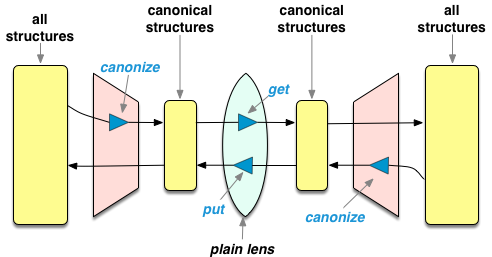
\includegraphics[width=0.7\textwidth]{canonizers-outside}
\caption{Quotient Lens with ``Canonizers at the Edges''
\sam{We don't need a general choose function. With QREs the kernel language is
always contained in the whole language so we just use the inclusion as the
choose function.}\bcp{Done.  But I wonder if the picture should mention QREs
explicitly, somehow... any ideas?}}\sam{Maybe we can put all structures, the
canonizer and the canonical strcutre in a box that says QRE?}\bcp{Like this?
 (But maybe we should go a step further and label things like $K(c)$,
 $W(c)$, Canonizer(c), etc.  And probably we should display K as a subset of
 W.  I can make these changes later.)}
\label{fig:attheedges}
\end{figure}
Every QRE lens $q$ has a type $q: c_1 \Leftrightarrow c_2$ where $c_1$ and $c_2$
are QREs. In the get direction, a QRE lens $q: c_1 \Leftrightarrow c_2$ uses the
source QRE $c_1$ to compute a unique representative for the data modulo the
equivalence relation defined by $c_1$ and then applies the $\get$ function of a
bijective lens $\ell$ to this representative. In the backward direction, $q$
operates similarly, but using the view QRE $c_2$ and the $\lput$ function of
$\ell$.

Because the QREs $c_1$ and $c_2$ determine the internal formats for data after
canonization, and because the algorithm for synthesizing bijective lenses is
directed by these formats, $c_1$ and $c_1$ are all that is required to
synthesize QRE lenses end-to-end. Indeed, we structured QRE lenses as bijective
lenses with canonizers at the edges, precisely to facilitate the use of this
synthesis algorithm.

On the other hand, our restriction that canonizers appear only at the edges
raises a key technical question:  Are we limiting the expressiveness of our
transformations by demanding all programs fit into this normal form?\bcp{I wish
we could have previewed this issue a bit more in the introduction, since it is
our main contribution.}  It turns out that we are not: any lens that uses
canonizers internally can be transformed into a lens that uses canonizers at
the edges. The main technical contribution of this paper is a proof of this
fact.

This technical investigation justifies replacing manually constructed lenses
using the QRE lens combinators with synthesized QRE lenses in normal form, thus
saving the programmer. For instance, after defining the \bibtex{} and EndNote
QREs and storing them in the variables \cd{bibtex} and \cd{endnote}
respectively, then all the code in Figure~\ref{fig:example-lens} may be
replaced by a single call to the synthesis prodedure:

\begin{lstlisting}
let bib_to_end : (lens in bibtex $\Leftrightarrow$ endnote) =
synth bibtex $\Leftrightarrow$ endnote using {(bib_example, end_example)}
\end{lstlisting}
\bcp{Again, the spacing is weird}
\noindent Here, the generated  quotient lens synchronizes \cd{bibtex} and
\cd{endnote} formats, using \cd{bib_example} and \cd{end_example} (the two
concrete example strings given at the beginning of this section) to
disambiguate. In addition, and as we saw earlier with the definition of
\cd{s_to_c}, the synthesis procedure itself can be used to create lenses that
are in turn used to define other QREs.  The ability to intermix QRE
specification with QRE lens synthesis yields a powerful and flexible way of
creating bidirectional transformations.

\section{Quotient Regular Expressions}
\label{QRE}
\subsection{Syntax and Semantics of QREs}
Formally, the language of Quotient Regular Expressions (QREs) is given by the
following grammar:
\begin{align*}
c := \; &R \sep \project{R}{s} \sep \squash{c_1}{c_2}{f} \sep
\perm{c_1, \ldots, c_n}{c} \\
& | \; \normalize{R}{R'}{f} \sep c_1 \semicolon c_2 \sep c_1 \cdot c_2 \sep (c_1
\sep c_2) \sep c^*,
\end{align*}
where $c$ ranges over QREs, $R$ ranges over regular expressions, $f$ ranges over
functions between regular languages, and $s$ ranges over character strings.

Using the conventional notation that $\mathcal{L}(R)$ is the language accepted
by the regular expression $R$, then each QRE $c$ enables us to express
\begin{enumerate}
  \item a regular expression $W(c)$ (the ``whole'' of $c$),
  \item an equivalence relation $\eqrel{c}$ on $\mathcal{L}(W(c))$,
  \item a regular expression $K(c)$ (the ``kernel'' of $c$)
  such that $\mathcal{L}(K(c))$ forms a complete set of representatives for
  $\eqrel{c}$, and
  \item a ``canonizing'' function $\canonizer(c):\mathcal{L}(W(c))
  \longrightarrow \mathcal{L}(K(c))$ which given any $w \in \mathcal{L}(W(c))$,
  computes $\canonizer(c)(w)$ as the unique $k$ in $\mathcal{L}(K(c))$ such that
  $k$ is equivalent to $w$ mod $\eqrel{c}$
\end{enumerate}
Figures~\ref{fig:wk} gives the inductive definitions for the whole and
kernel languages $W(c)$ and $K(c)$ of a QRE.
\begin{figure}[t]
\centering
\[
\begin{array}{l@{\quad}l@{\quad}l}

c & W(c) & K(c) \\ \hline
R & R & R \\
\project{R}{s} & R & s \\
\squash{c}{c_1}{f} & W(c) \sep W(c_1) & K(c_1) \\
\normalize{R}{R'}{f} & R & R' \\
c_1 \; ; \; c_2 & W(c_1) & K(c_2) \\
c_1 \cdot c_2 & W(c_1) \cdot W(c_2) & K(c_1) \cdot K(c_2) \\
c_1 \sep c_2 & W(c_1) \sep W(c_2) & K(c_1) \sep K(c_2) \\
c^* & W(c)^* & K(c)^* \\
\end{array}
\]
\[
\begin{array}{r@{\quad}l}
W( \perm{c_1, \ldots, c_n}{c} ) = &
\bigcup \limits_{\sigma \in S_n} W(c_{\sigma(1)}) \cdot W(c) \cdot \ldots \cdot
W(c) \cdot W(c_{\sigma(n)})\\
K( \perm{c_1, \ldots, c_n}{c} ) = & K(c_1) \cdot K(c) \cdot \ldots \cdot K(c)
\cdot K(c_n)
\end{array}
\]
\caption{Whole and Kernel Regular Expressions}
\label{fig:wk}
\end{figure}
The \textit{squash} and \textit{permutation} combinators give the two
interesting definitions. If $c = \squash{c}{c_1}{f}$, then the whole language of
$c$ is $W(c) \sep W(c_1)$. This is because the \textit{squash} combinator takes
the whole language $W(c)$ of $c$, the whole language $W(c_1)$ of $c_1$ and a
function $f : \mathcal{L}(W(c)) \longrightarrow \mathcal{L}(W(c_1))$, maps
$\mathcal{L}(W(c))$ into $\mathcal{L}(W(c_1))$ using $f$ and then canonizes
$W(c_1)$ into $K(c_1)$ using $\canonizer(c_1)$.

For the $\perm{c_1, \ldots, c_n}{c}$ combinator, the whole language is the
union of languages of the form $W(c_{\sigma(1)}) \cdot W(c) \cdot \ldots \cdot
W(c) \cdot W(c_{\sigma(n)})$ for any permutation $\sigma$ in $S_n$, where
$S_n$ is the set of all permutations of the numbers $1$ to $n$. This is because
the \textit{permutation} combinator allows for the string to match any
permutation the $c_i$'s while also taking into account the separator $c$ in
between each of the $c_i$'s. The kernel of the \textit{permutation} combinator
is the language $K(c_1) \cdot K(c) \cdot \ldots \cdot K(c) \cdot K(c_n)$,
because the canonical permutation is the identity permuation, with each of the
parts of the string that match $c_i$ and $c$ canonized into $K(c_i)$ and $K(c)$
respectively.

Figure~\ref{fig:canonizers} gives the inductive definitions of the
$\canonizer{}$ function for each QRE.
\begin{figure}[t]
\begin{center}
\[
\begin{array}{l@\quad l @\quad l}
\canonizer(R) &=& id_{\mathcal{L}(R)} \\
\canonizer(\project{R}{s})(w) &=& s\\
\canonizer(\squash{c_1}{c_2}{f})(w) &=&
\begin{cases}
\canonizer(c_1)(f(w)) & \text{if } w \in \mathcal{L}(W(c_1))\\
\canonizer(c_2)(w) & \text{otherwise}
\end{cases}\\
\canonizer(\normalize{R}{R'}{f}) &=& f\\
\canonizer(c_1 \; ; \; c_2) &=& \canonizer(c_2) \circ \canonizer(c_1)\\
\canonizer(c_1 \cdot c_2) &=& \canonizer(c_1) \cdot \canonizer(c_2)\\
\canonizer(c_1 \sep c_2)(w) &=&
\begin{cases}
\canonizer(c_1)(w) & \text{if } w \in \mathcal{L}(W(c_1))\\
\canonizer(c_2)(w) & \text{if } w \in \mathcal{L}(W(c_2))\\
\end{cases}\\
\canonizer(c^*) &=& \canonizer(c)^* \\
\end{array}
\]
\end{center}
\begin{align*}
&\canonizer(\perm{c_1, \ldots, c_n}{c})(r_{\sigma(1)}
\cdot s_1 \cdot \ldots \cdot s_{n-1} \cdot r_{\sigma(n)})\\
&= (\canonizer(c_1)(r_1)) \cdot (\canonizer(c)(s_1)) \cdot \ldots \cdot
(\canonizer(c_n)(r_n))
\end{align*}
\caption{QRE canonizers}
\label{fig:canonizers}
\end{figure}
Again, the \textit{permutation} combinator gives the most interesting
definition,
\begin{align*}\canonizer(\perm{c_1, \ldots, c_n}{c})(r_{\sigma(1)}
\cdot s_1 \cdot \ldots \cdot s_{n-1} \cdot r_{\sigma(n)}) \\
= (\canonizer(c_1)(r_1)) \cdot (\canonizer(c)(s_1)) \cdot \ldots \cdot
(\canonizer(c_n)(r_n))
\end{align*}
\noindent which as we have explained is defined so that the strings that match
$c_i, c$ are placed in the canonical permutation which is the identity
permutation before $\canonizer(c_i)$ and $\canonizer(c)$ are applied
respectively.

Finally, Figure ~\ref{fig:relations} gives the induction defintion of the
equivalence relation $\eqrel{c}$. These are the set-theoretic semantics of QREs
as an equivalence relation on a regular language.

\begin{figure}[t]
\centering
\[
\begin{array}{l@{\quad}l@{\quad}l}
w \; \equiv_R \; w' &\iff& w = w' \\
w \; \equiv_{\project{R}{s}} \; w' \text{ for all }w, w'\\
w \; \equiv_{\squash{c_1}{c_2}{f}} \; w' &\iff& f(w) \equiv_{c_2} w'
\text{ or } w \equiv_{c_2} w' \\
w \; \equiv_{\normalize{R}{R'}{f}} \; w' &\iff&
f(w)=f(w') \text{ or }w = w'\\
w \; \equiv_{c_1 \; ; \; c_2} \; w' &\iff& \exists k, k' \in
\mathcal{L}(K(c_2)) \text{ such that } w \; \equiv_{c_1} \; k, \; w' \;
\equiv_{c_1} \; k', \text{ and } k \; \equiv_{c_2} \; k'\\
w \; \equiv_{c_1 \cdot c_2} \; w'  &\iff& w = r_1
\cdot r_2, \; w' = {r'}_1 \cdot {r'}_2 \text{ with } r_1 \; \equiv_{c_1}
\; {r'}_1, \; r_2 \; \equiv{c_n} \; {r'}_2\\
w \; \equiv_{c_1 \sep c_2} \; w' &\iff& w \; \equiv_{c_1} \; w'
\text{ or } \; w \; \equiv_{c_2} \; w'\\
w \; \equiv_{c^*} \; w' &\iff& w = r_1 \cdot \ldots \cdot r_n, \; w'
= {r'}_1 \cdot \ldots \cdot {r'}_n \text{ and } r_i \equiv_{c} \; {r'}_i
\\
w \; \equiv_{\perm{c_1, \ldots, c_n}{c}} \; w' &\iff& w = r_{\sigma(1)}
\cdot s_1 \cdot \ldots \cdot s_{n-1} \cdot r_{\sigma(n)}, \;
w' = {r'}_{\theta(1)} \cdot s'_1 \cdot \ldots \cdot s'_{n-1}
\cdot {r'}_{\theta(n)} \\
& & \text{ for some } \sigma, \theta \in S_n, \text{ with } r_i \;
\equiv_{q_i} \; r'_i \text{ and } s_k \; \equiv_{c} \; s'_{k}
\end{array}
\]
\caption{QRE Equivalence Relations}
\label{fig:relations}
\end{figure}
\subsection{Ambiguity and Well Formed QREs}
Before giving the inference rules for deriving well formed QREs, we address
the issue of {\em ambiguity}, which appears in the premises of the inference
rules for the regular combinators. If $c$ and $c_1$ are QREs, then when applying
the regular combinators to QREs, we require that if a string $s$ matches any of
the regular expressions $W(c) \cdot W(c_1)$, \quad $W(c) \sep W(c_1)$,
\quad $W(c)^*$, \quad $K(c) \cdot K(c_1)$, \quad $K(c) \sep K(c_1)$,
\quad $K(c)^*$, then $s$ matches that regular expression in only one way. 

More formally, we say that regular expressions $R$ and $S$ are
\textit{unambiguosly concatenable}, written $R \cdot^! S$ if for all strings
$r, r' \in \mathcal{L}(R)$ and $s, s' \in \mathcal{L}(S)$, if $r \cdot s = r'
\cdot s'$, then $r = r'$ and $s = s'$. We say that a regular expression $R$ is
\textit{unambiguosly iterable}, written $R^{*!}$ if for all strings $r_1,
\ldots, r_m$ and $r'_1, \ldots, r'_n \in \mathcal{L}(R)$, if $r_1 \cdot \ldots
\cdot r_m = r'_1 \cdot \ldots \cdot r'_n$, then $m = n$ and $r_i = r'_i$. We say
that a regular expression $R$ is \textit{strongly unambiguous}\cite{Sippu1988}
if and only if (1) $R = \varnothing$, or (2) $R = S_1 \cdot S_2$ with $S_1,
S_2$ strongly unambiguous and $S_1 \cdot^! S_n$, or (3) $R = S_1 \sep S_2$ with
$S_1, S_2$ strongly unambiguous and $\mathcal{L}(S_1) \cap \mathcal{L}(S_2) =
\varnothing$, or (4) $R = S^*$ with $S$ strongly unambiguous and $S^{*!}$.

Strong unambiguity is necessary in the premises of the regular QRE combinators
because it ensures that the canonizing function of a QRE is well-defined.
For example consider the QRE \lstinline{"a"* . (project "a"* $\to$ "a")}. The
behaviour of this QRE is not-well defined since the string
\cd{"aaa"} can be canonized to any of \cd{"a"}, \cd{"aa"}, or \cd{"aaa"}
depending on how \cd{"aaa"} is parsed. We also require that the regular
combinators applied to the kernels of QREs be unambiguous since the underlying
bijective lens of a QRE lens operates on kernels, and bijective lenses
impose the same unambiguity restrictions so that they too are well defined as
functions.

Figure~\ref{fig:qrerules} gives the inferrence rules for deriving well-formed
QREs.
\begin{figure}[tp!]
\begin{center}
\AxiomC{$R$ is strongly unambiguous}
\UnaryInfC{$\wf{\mathit{id}(R)}$}
\DisplayProof
\hskip 1.5em
\AxiomC{$s \in \mathcal{L}(R)$}
\UnaryInfC{$\wf{\project{R}{s}}$}
\DisplayProof
\hskip 1.5em
\end{center}

\begin{prooftree}
\AxiomC{$\wf{c_i, c}$}
\AxiomC{${\substack{\forall \sigma \neq \theta, \; W(c_{\sigma(1)}) \cdot W(c)
\cdot \ldots \cdot W(c_{\sigma(n)})\\ \cap W(c_{\theta(1)}) \cdot W(c)
\cdot \ldots \cdot W(c_{\theta(n)}) =\varnothing}}$}
\AxiomC{$K(c_1) \cdot^! K(c) \cdot^! \ldots \cdot^! K(c) \cdot^! K(c_n)$}
\TrinaryInfC{$\wf{\perm{c_1, \ldots, c_n}{c}}$}
\end{prooftree}

\begin{center}
\AxiomC{$\wf{c_1, c_2}$}
\AxiomC{$\mathcal{L}(W(c_1)) \cap \mathcal{L}(W(c_2)) = \varnothing$}
\AxiomC{$f : \mathcal{L}(W(c_1)) \longrightarrow \mathcal{L}(W(c_2))$}
\TrinaryInfC{$\wf{\squash{c_1}{c_2}{f}}$}
\DisplayProof
\end{center}
\begin{center}

\begin{prooftree}
\AxiomC{$\mathcal{L}(R') \subseteq \mathcal{L}(R)$}
\AxiomC{$f : \mathcal{L}(R) \longrightarrow \mathcal{L}(R')$}
\AxiomC{$f$ is surjective}
\AxiomC{$f = f^2$}
\QuaternaryInfC{$\wf{\normalize{R}{R'}{f}}$}
\end{prooftree}

\end{center}
\begin{center}
\AxiomC{$\wf{c_1, c_2}$}
\AxiomC{$K(c_1) = W(c_2)$}
\BinaryInfC{$\wf{c_2 \; ; \; c_1}$}
\DisplayProof
\hskip 1.5em
\AxiomC{$\wf{c}$}
\AxiomC{$W(c)^{*!}$}
\AxiomC{$K(c)^{*!}$}
\TrinaryInfC{$\wf{c^*}$}
\DisplayProof
\end{center}
\begin{center}

\begin{center}
\AxiomC{$\wf{c_1, c_2}$}
\AxiomC{$W(c_1) \cdot^! W(c_2)$}
\AxiomC{$K(c_1) \cdot^! K(c_2)$}
\TrinaryInfC{$\wf{c_1 \cdot c_2}$}
\DisplayProof
\end{center}

\begin{center}
\AxiomC{$\wf{c_1, c_2}$}
\AxiomC{$W(c_1) \cap W(c_2) = \varnothing$}
\BinaryInfC{$\wf{c_1 \cdot c_2}$}
\DisplayProof
\hskip 1.5em
\AxiomC{$\wf{c}$}
\AxiomC{$W(c)^{*!}$}
\AxiomC{$K(c)^{*!}$}
\TrinaryInfC{$\wf{c^*}$}
\DisplayProof
\end{center}
\end{center}
\caption{Well-formed QREs
}
\label{fig:qrerules}
\end{figure}
As we already mentioned, the unambiguity conditions come into play when defining
QREs using the regular combinators. For example, the inferrence rule for
concatenation is as follows:\bcp{Rather than repeating rules inline, give
  them names in the figure.}
\begin{prooftree}
\AxiomC{$\wf{c, c_1}$}
\AxiomC{$W(c) \cdot^! W(c_1)$}
\AxiomC{$K(c) \cdot^! K(c_1)$}
\TrinaryInfC{$\wf{c \cdot c_1}$}
\end{prooftree}

\noindent This rule says that the concatenation $c \cdot c_1$ of QREs $c$ and
$c_1$ is well formed only if the concatentions of $W(c)$ and $W(c_1)$, and
$K(c)$ and $K(c_1)$ are unambiguous.

The most complicated inferrence rule is the rule for the \textit{permutation}
combinator:

\begin{prooftree}
\AxiomC{$\wf{c_i, c}$}
\AxiomC{${\substack{\forall \sigma \neq \theta, \; W(c_{\sigma(1)}) \cdot W(c)
\cdot \ldots \cdot W(c_{\sigma(n)})\\ \cap W(c_{\theta(1)}) \cdot W(c)
\cdot \ldots \cdot W(c_{\theta(n)}) =\varnothing}}$}
\AxiomC{$K(c_1) \cdot^! K(c) \cdot^! \ldots \cdot^! K(c) \cdot^! K(c_n)$}
\TrinaryInfC{$\wf{\perm{c_1, \ldots, c_n}{c}}$}
\end{prooftree}

\noindent The second hypothesis for the \textit{permutation} rule says that for
any two different permutations $\sigma$ and $\theta$, the languages
$W(c_{\sigma(1)}) \cdot W(c) \cdot \ldots \cdot W(c_{\sigma(n)})$ and
$W(c_{\theta(1)}) \cdot W(c) \cdot \ldots \cdot W(c_{\theta(n)})$ must be
disjoint. This is because any string that matches the \textit{permutation}
combinator matches the language $W(c_{\theta(1)}) \cdot W(c) \cdot \ldots \cdot
W(c_{\theta(n)})$ for some permutation $\theta$, so we require that these
regular expressions be disjoint.

The third hypothesis says that the regular expression $K(c_1) \cdot K(c)
\cdot \ldots \cdot K(c) \cdot K(c_n)$ must be unambiguous. This is because the
underlying lens that maps to or from a \textit{permutation} QRE operates on
the language $K(c_1) \cdot K(c) \cdot \ldots \cdot K(c) \cdot K(c_n)$ which is
the kernel of the \textit{permutation} QRE. As we mentioned, the underlying
lens will require that the source and target regular expressions of the lens be
unambiguous so that the lens can match strings uniquely.

At this point we also bring to attention the fact that in order for the {\em
normalize} QRE to be well-formed, then canonizing function $f$ used by this
combinator must be surjective and idempotent. Unfortunately, verifying
that a function satisfies these properties is in general undecidable.
Nonetheless, we allow a programmer to use normalize at their own risk without
checking these side conditions.

We do this firstly because the {\em normalize} combinator allows one to express
equivalence relations that are either difficult to define, or that cannot be
defined using the other combinators. Secondly, the {\em normalize} canonizer
enjoys the property that each of the other combinators $c$ is semantically
equivalent to $\normalize{W(c)}{K(c)}{f}$ for some surjective, idempotent
function $f : \mathcal{L}(W(c)) \longrightarrow \mathcal{L}(K(c))$. The {\em
normalize} combinator hence gives a sufficient condition for potential QREs to
be ``well-behaved'', particularly with respect to the strategy for synthesizing
quotient lenses which we shall introduce in Section~\ref{synth}.  \bcp{I
  think here we're mixing concerns of language design with the concerns of
  the underlying theory.  Indeed, I think it would be clearer to reorganize
  the whole section as follows: first present just normalize and discuss its
  properties; then observe that the side condition is annoying because it
  cannot be checked automatically; then introduce project, squash, and perm
  as a pragmatically motivated, extensible set of safe combinators that
  we've found useful for a broad range of examples.  This will also help
  address the complaint that extracting half of a lens is a hack.}

In spite of this ``completeness'' property of the {\em normalize} combinator,
our experience with QREs shows that using the {\em project}, {\em squash} and
{\em perm} combinators as well as the regular operators applied to these is
much easier than using just {\em normalize} because of the compositional nature
of the other combinators.  \bcp{Maybe this comment is not needed?  It seems
  obvious, besides the fact that these other combinators are safe while
  normalize requires a proof by hand.}

The formal semantics of QREs satisfy the following theorem:\bcp{That bit is
  entirely redundant with the theorem itself.  Either simply delete it or
  replace with something more interesting. :-)}
\begin{theorem}
If $c$ is a well formed QRE, then
\begin{enumerate}
  \item $W(c)$ and $K(c)$ are well defined regular expressions,
  \item  $\eqrel{c}$ is an equivalence relation on $\mathcal{L}(W(c))$,
  \item  $\mathcal{L}(K(c))$ forms a complete set of representatives for
  $\eqrel{c}$,
  \item $\canonizer(c):\mathcal{L}(W(c)) \longrightarrow \mathcal{L}(K(c))$ is
  a well-defined function, and
  \item  given any $w \in \mathcal{L}(W(c))$, $\canonizer(c)(w)$ is the unique
  $k$ in $\mathcal{L}(K(c))$ such that $k$ is equivalent to $w$ modulo
  $\eqrel{c}$.
\end{enumerate}
\end{theorem}

\section{QRE Lenses}
\label{QRE-lenses}
As we have seen, QREs express a broad class of equivalence relations
directly on regular languages.  QREs are therefore a good \textit{specification}
language for quotient lenses. We next introduce
\textit{QRE Lenses}, a class of quotient lenses specified using QREs.

\bcp{A question about variable names: If we use $R$ and $S$ for plain
  regular expressions, it seems inconsistent to use $c$ for QREs.  (And even
  more inconsistent to use $c$ and $c'$ or $c$ and $c_1$!) I suggest $P$ and
  $Q$ for QREs (with $Q$ as the default when we are only talking about
  one).}

Given regular expressions $R, S$ and equivalence relations
$\sim_R$ and $\sim_S$ defined on $\mathcal{L}(R)$ and $\mathcal{L}(S)$
respectively, we\bcp{can we clarify that this is exactly Foster et al's definition?} define a {\em bijective quotient lens} $q : R /{\sim_R}
\Leftrightarrow S/{\sim_S}$ to be a pair of functions $q.get :
\mathcal{L}(R) \longrightarrow \mathcal{L}(S)$ and $q.put : \mathcal{L}(S)
\longrightarrow \mathcal{L}(R)$ such that for all $r \in \mathcal{L}(R)$ and $s
\in \mathcal{L}(S)$,
\begin{align*}
q.put(q.get(r)) &\sim_R r \text{, and}\\
q.get(q.put(s)) &\sim_R s
\end{align*}
Moreover, if $r \sim_R r'$, then $q.get(r) = q.get(r')$, and if $s \sim_S s'$,
then $q.put(s) = q.put(s')$.  \bcp{We should emphasize that this is
  precisely the desired loosening of the too-strict plain lens laws.}

In words, a bijective quotient lens $q$ from $R$ to $S$ modulo $\sim_R$
and $\sim_S$ is a pair of functions $q.get$ and $q.put$ such that $q.get$
respects $\sim_R$ and $q.put$ respects $\sim_S$, and such that the $get$ and
$put$ functions lifted to $\mathcal{L}(R)/{\sim_R}$ and
$\mathcal{L}(S)/{\sim_S}$ are mutual inverses.

\bcp{Typesetting: $q.get$ and $q.\get$ are subtly different, as are
  $q.put$ and $q.\lput$, and the latter forms are the correct ones.
  In general, you should never put a whole word in math mode without
  wrapping it in mathit: the inter-letter spacing will be wrong.}

Now let $c$ and $c_1$ be QREs. Given a bijection $\ell : K(c) \Leftrightarrow
K(c_1)$, we may define a quotient lens $q : W(c)/\eqrel{c} \Leftrightarrow
W(c_1)/\eqrel{c_1}$ by
\begin{equation}\label{normalform}
q.get = \ell \circ \canonizer(c) \text{ and } q.put = \ell^{-1} \circ
\canonizer(c_1),
\end{equation}

\noindent In other words, the get function of the $q$ first canonizes the source
data using $\canonizer(c)$ and then applies $f$ to the result, while the
put function of the $q$ first canonizes the target data using
$\canonizer(c_1)$ and the applies $f^{-1}$ to the result. This is our approach in
defining QRE lenses.

One potential pitfall with QRE lenses is that the combinators that
we define on them may not preserve this normal form. For example, the
composition $q' \; ; \; q$ of QRE lenses $q$ and $q'$ may not be equivalent to
any quotient lens that has the canonical normal form of a bijective lens with
canonizers a the edges. Consequently, in order to guarantee that every QRE
lens $q$ is equivalent to a QRE lens $q'$ which has the canonical form of
a bijection with canonizers at the edges, we need to identify a set $S$ of
bijections that will ensure that QRE lenses are closed under the action of QRE
lens combinators. Our choice is to use the class of \textit{bijective lenses},
which we briefly discuss in the next section.

\subsection{Bijective Lenses}
We define the set of \textit{bijective lenses} to be the set of bijections
between regular languages created using Boomerang lens combinators.
The syntax for the language of bijective lenses is given by
$$\ell := \mathit{id} \; (R) \sep const(s, s') \sep  swap(\ell,
\ell) \sep \ell \cdot \ell' \; |  \; (\ell \sep \ell') \sep \ell^* \;
| \; \ell \circ \ell',$$ where $R$ ranges over regular expressions and $s$
ranges over character strings.

The denotation of a lens $\ell$ is $\llbracket \ell \rrbracket \subseteq
\mathit{String} \times \mathit{String}$. If $(s_1, s_2) \in \llbracket \ell
\rrbracket$, then $\ell$ maps between $s_1$ and $s_2$.
\begin{align*}
\llbracket R \rrbracket &= \{(r, r) \sep r \in \mathcal{L}(R)\}\\
\llbracket const(r, s) \rrbracket &= \{(r, s)\}\\
\llbracket swap(\ell, \ell') \rrbracket &= \{(s \cdot t, t' \cdot s') \sep
(s, s') \in \llbracket \ell \rrbracket \text{ and } (t, t') \in \llbracket
\ell' \rrbracket\}\\
\llbracket \ell \cdot \ell' \rrbracket &= \{(s \cdot t, s' \cdot t) \sep
(s, s') \in \llbracket \ell \rrbracket \text{ and } (t, t') \in \llbracket
\ell' \rrbracket\}\\
\llbracket \ell \sep \ell' \rrbracket &= \{(s \cdot t) \sep
(s, t) \in \llbracket \ell \rrbracket \text{ or } (s, t) \in \llbracket
\ell' \rrbracket\}\\
\llbracket \ell^* \rrbracket &= \{(s_1 \cdot \ldots \cdot s_n, t_1 \cdot \ldots
\cdot t_n) \sep (s_i, t_i) \in \llbracket \ell \rrbracket \text{ for } 1
\leq i \leq n\}\\
\llbracket \ell_2 \circ \ell_1 \rrbracket &= \{(r, t) \sep \text{there exists }s
\text{ such that } (r, s) \in \llbracket \ell_1 \rrbracket \text{ and } (s, t)
\in \llbracket \ell_2 \rrbracket\}
\end{align*}
The $\mathit{const}(s, t)$ lens replaces the string $s$ with $t$ in the source
data in the forward direction, and $t$ with $s$ in the target data in the backward
direction. $\mathit{id}(R)$ applies the identity function to the source and target
in $\mathcal{L}(R)$ in both directions. The composition lens $\ell' \circ \ell$
applies $\ell$ followed by then $\ell'$ to the source in the forward direction,
and applies $\ell'$ followed by $\ell$ to the target in the backward direction.
The lens $\ell \cdot \ell'$ first splits the string $s$ into $s_1$ and $s_2$,
applies $\ell$ and $\ell'$ to $s_1$ and $s_2$ to get $t_1$ and $t_2$
respectively, then concatenates $t_1$ and $t_2$ and returns $t_1 \cdot t_2$ as
the final result in the forward direction. $\ell \cdot \ell'$ operates
similarly in the backward direction, but with $s, s_1$ and $s_2$ substituted
for $t, t_1$ and $t_2$. The $\mathit{swap} \; (\ell, \ell')$ lens operates
like $\ell \cdot \ell'$, except that it swaps $t_1$ and $t_2$ before
concatenating the two for a final result of $t_2 \cdot t_1$ in the forward
direction. In the backward direction, $\mathit{swap}(\ell, \ell')$ first undoes
the swap, then proceeds as expected. The $\ell \; | \; \ell'$ lens
chooses to apply $\ell$ or $\ell'$ depending on whether the source
(resp. target) data is matched by $\ell$ or $\ell'$ in the forward (resp.
backward direction). The $\ell^*$ lens splits the string $s$ into strings $s_1,
\ldots, s_n$, applies $\ell$ to each $s_i$ to get $t_i$, and then concatenates
each of the $t_i$'s for a final result of $t_1 \cdot \ldots \cdot t_n$ in the
forward direction. $\ell^*$ operates similarly in the backward direction, but
with $s, s_i$ substituted for $t, t_i$.

Each bijective lens $\ell$ has a type $\ell : R \Leftrightarrow S$ where $R$ and
$S$ are regular expressions. If $\ell : R \Leftrightarrow S$, then the source
language of $\ell$ is $\mathcal{L}(R)$ and the target language of $\ell$ is
$\mathcal{L}(S)$. Interestingly, with the bijective lens type system, a lens
$\ell : R \Leftrightarrow S$ can also be considered to be of type $\ell : R'
\Leftrightarrow S'$ provided that $R$ (resp. $S$) can be proven to be
equivalent to $R'$ (resp. $S$) from the star-semiring axioms:

\begin{prooftree}
\AxiomC{$\ell : R \Leftrightarrow S$}
\AxiomC{$R \equiv^s R'$}
\AxiomC{$S \equiv^s S'$}
\TrinaryInfC{$\ell : R' \Leftrightarrow S'$}
\end{prooftree}

The other typing rules for bijective lenses are given in
Figure~\ref{fig:lensrules}.

\begin{figure}[t]
\begin{center}
\AxiomC{$s_1 \in \Sigma^*$}
\AxiomC{$s_2 \in \Sigma^*$}
\BinaryInfC{$\mathit{const} \; (s_1, s_t): s_1 \Leftrightarrow s_2$}
\DisplayProof
\hskip 1.5em
\AxiomC{$R$ is strongly unambiguous}
\UnaryInfC{$\mathit{id} \; (R): R \Leftrightarrow R$}
\DisplayProof
\end{center}

\begin{center}
\AxiomC{$\substack{\ell_1 : R_1 \Leftrightarrow S_1 \\ \ell_2 : R_2
\Leftrightarrow S_2}$}
\AxiomC{$\substack{R_1 \cdot^! R_2 \\S_1 \cdot^! S_2 }$}
\BinaryInfC{$\ell_1 \cdot \ell_2: R_1 \cdot R_2 \Leftrightarrow S_1 \cdot
S_2$}
\DisplayProof
\hskip 1.5em
\AxiomC{$\substack{\ell_1 : R_1 \Leftrightarrow S_1 \\ \ell_2 : R_2
\Leftrightarrow S_2}$}
\AxiomC{$\substack{R_1 \cdot^! R_2 \\ S_2 \cdot^! S_1}$}
\BinaryInfC{$\mathit{swap} \; (\ell_1, \ell_2): R_1 \cdot R_2
\Leftrightarrow S_2 \cdot S_1$}
\DisplayProof
\end{center}

\begin{center}
\AxiomC{$\ell_1 : R_1 \Leftrightarrow R_2$}
\AxiomC{$\ell_2 : R_2 \Leftrightarrow R_3$}
\BinaryInfC{$\ell_2 \circ \ell_1: R_1 \Leftrightarrow R_3$}
\DisplayProof
\hskip 1.5em
\AxiomC{$\substack{\ell_1 : R_1 \Leftrightarrow S_1 \\ \ell_2 : R_2
\Leftrightarrow S_2}$}
\AxiomC{$\substack{\mathcal{L}(R_1) \cap \mathcal{L}(R_2) =
\varnothing \\ \mathcal{L}(S_1) \cap \mathcal{L}(S_2) = \varnothing}$}
\BinaryInfC{$\ell_1 \sep \ell_2: R_1 \sep R_2 \Leftrightarrow S_1 \sep S_2$}
\DisplayProof
\end{center}

\begin{center}
\AxiomC{$\ell : R \Leftrightarrow S$}
\AxiomC{$R^{*!}$}
\AxiomC{$S^{*!}$}
\TrinaryInfC{$\ell^*: R \Leftrightarrow S$}
\DisplayProof
\hskip 1.5em
\AxiomC{$\ell : R \Leftrightarrow S$}
\AxiomC{$R \equiv^s R'$}
\AxiomC{$S \equiv^s S'$}
\TrinaryInfC{$\ell : R' \Leftrightarrow S'$}
\DisplayProof
\end{center}
\caption{Bijective Lens Typing Rules}
\label{fig:lensrules}
\end{figure}

\subsection{Syntax of QRE Lenses}
Having given a brief overview of the class of bijective lenses, we now introduce
the class of QRE lenses. The language of QRE lenses is given by following
grammar:
$$ q := \kw{lift}(\ell) \sep \kw{lquot}(q, \ell) \sep
\kw{rquot}(\ell, q) \sep q \cdot q' \sep (q \sep q') \sep q^* \sep q \circ q',$$
where $\ell$ ranges over bijective lenses.

The QRE lens combinators are inspired by the Boomerang lens combinators of the
same name. The $\kw{lift}(\ell)$ quotient lens enables a bijective lens
$\ell$ to be considered a quotient lens, with the equivalence relation applied
to both the source and target formats being the equality relation. The
regular combinators of concatenation `$\cdot$', Kleene star `$*$' and
`$|$' on QRE lenses exhibit the expected behaviour, with the caveat that these
combinators are strongly unambiguous. The composition operator `$;$' also
exhibits the expected behaviout, though the conditions that must be checked in
order for the composition to be well defined are perhaps unintuitive. The
reasons why these conditions are necesary will become more apparent when
proving normal forms for QRE lenses.

The interesting combinators are the $\kw{lquot}$ and $\kw{rquot}$
combinators. The $\kw{lquot}(c, q)$ combinator takes a quotient lens $q$ and
quotients the source data using $c$, assuming that the source data forms a
complete set of representatives for the equivalence relation $\eqrel{c}$. The
$\kw{lquot}(q, c)$ combinator does the same but on the target data.

For example, recall that in the \bibtex{} to EndNote transformation, we had the
QREs \cd{bibtex} and \cd{endnote} describing the \bibtex{} and EndNote records
respectively, and the bijective lens \cd{bib_to_end} that maps between
\cd{bibtex} and \cd{endnote}. The quotient lens that maps between
\cd{bibtex} and \cd{endnote} is given by the QRE lens

\begin{lstlisting}
let bib_to_end_q : (lens in bibtex $\Leftrightarrow$ endnote)  = rquot (lquot(bibtex, bib_to_end), endnote)
\end{lstlisting}

\iffalse
The difference between QRE lenses and Boomerang quotient lenses lies in the
typing judgements. More concretely, each QRE lens $q$ has a type $q : c
\Leftrightarrow c_1$ where $c, c_1$ are QREs. In contrast, the approach used to
type quotient lenses in Boomerang is to classify equivalences according to
whether they are or are not the equality relation. This type system is based on
two observations: first, that most quotient lenses originate as lifted basic
lenses, and therefore have types whose equivalence relations are both equality;
and second, that equality is preserved by many of the quotient lens
combinators. Foster et al also discuss a second possible approach to typing
quotient lenses, where equivalence relations are represented by rational
functions that induce them. While this second approach is more refined than the
first, Boomerang favours the first approach since the second appears to be too
expensive to be useful in practice~\cite{quotientlenses}.
\fi

\subsection{Semantics of QRE Lenses}

Each QRE lens $q$ has a type $q : c \Leftrightarrow c_1$ where $c, c_1$ are QREs.
If $q : c \Leftrightarrow c_1$, then the source format is described by $W(c)$ and
the canonical set of representative for the source data is described by $K(c)$.
Similarly, the target format is described by $W(c_1)$ and the canonical set of
representatives for the target data is described by $K(c_1)$. The underlying lens
of $q$ is a bijective lens $\ell : K(c) \Leftrightarrow K(c_1)$.

The denotation $\llbracket q \rrbracket$ of a QRE lens $q:c \Leftrightarrow c_1$
is a quotient lens $\llbracket q \rrbracket : W(c)/{\eqrel{c}}
\Longleftrightarrow W(c_1)/{\eqrel{c_1}}$. The typing rules and denotation of QRE
lenses are given in Figure~\ref{fig:qlenssemantics}. The trickiest typing rule
is the typing rule for composition:

\begin{prooftree}
\AxiomC{$\substack{q_1 : c \Leftrightarrow c_1 \\ q_2 : c_2 \Leftrightarrow
c_3}$}
\AxiomC{$\substack{\mathcal{L}(W(c_1))= \mathcal{L}(W(c_2)) \\ K(c_1) \equiv
K(c_2)}$}
\AxiomC{$\canonizer(c_1) = \canonizer(c_2)$}
\TrinaryInfC{$q_2 \circ q_1: c \Leftrightarrow c_3$}
\end{prooftree}

This derivation rule essentially says that the composition $q_2 \circ q_1$ is
well defined if and only if the intermediary QREs $c_2$ and $c_3$ define the
same equivalence relation on the same regular language. The condition
$\mathcal{L}(W(c_1)) = \mathcal{L}(W(c_2))$ says that the intermediary language
is the same on both sides, while the condition $K(c_1) \equiv K(c_2)$ says that
the kernel regular expressions are syntactically the same. Finally, the
condition $\canonizer(c_1) = \canonizer(c_2)$ says that $c_1$ and $c_2$ define
the same equivalence relation on $\mathcal{L}(W(c_1))= \mathcal{L}(W(c_2))$.

In general, checking that $\canonizer(c_1) = \canonizer(c_2)$ is an undecidable
task, especially because of the $\normalize{R}{R'}{f}$ QRE. Therefore, our
actual implementation of the composition rule for QRE lenses follows Boomerang's
approach, which is to define the composition on QRE lenses if and only if
$c_1$ and $c_2$ are syntactially equal to $id(R)$ and $id(R')$ for some $R$ and
$R'$ satisfying $\mathcal{L}(R) = \mathcal{L}(R')$.

Foster et al based this approach on two observations: first, that most quotient
lenses originate as lifted basic lenses, and therefore have types whose
equivalence relations are both equality; and second, that equality is preserved
by many of the quotient lens combinators. Foster et al also discuss a second
possible approach, where equivalence relations are represented by rational
functions that induce them. While this second approach is more refined than the
first, Boomerang favours the first approach since the second appears to be too
expensive to be useful in practice~\cite{quotientlenses}.

The semantics defined on QRE lenses imply the following theorem:
\begin{theorem}
If there is a derivation $q : c \Leftrightarrow c_1$, then $\llbracket q
\rrbracket : W(c)/{\eqrel{c}} \Leftrightarrow W(c_1)/{\eqrel{c_1}}$ is a
well-defined quotient lens.
\end{theorem}


\begin{figure}[ht]
\centering
\[
\begin{array}[b]{l@{\qquad}l}
\Rule{\ell : R \Leftrightarrow S}{\kw{lift}(\ell): id(R) \Leftrightarrow id(S)}
&
\begin{array}[b]{rcl}
\llbracket \kw{lift}(\ell) \rrbracket.get &=&  \llbracket \ell \rrbracket\\
\llbracket \kw{lift}(\ell) \rrbracket.put &=& \llbracket \ell \rrbracket^{-1}
\end{array}
\end{array}
\]
\[
\begin{array}[b]{c@{\qquad}c}
\Rule{q : c_1  \Leftrightarrow c_2 &
\wf{c} &
K(c) = W(c_1)}
{\kw{lquot}(c, q): c_1 \circ c \Leftrightarrow c_2} &
\begin{array}[b]{rcl}
\llbracket \kw{lquot}(c, q) \rrbracket.get  &=& \llbracket q
\rrbracket.get \circ \canonizer(c)\\
\llbracket \kw{lquot}(c, q) \rrbracket.put &=& \llbracket q \rrbracket.put
\end{array}
\end{array}
\]

\[
\begin{array}[b]{c@{\qquad}c}
\Rule{q : c \Leftrightarrow c_2 &
\wf{c_2} &
W(c_2) = K(c_1)}
{\kw{rquot}(q, c):c \Leftrightarrow c_2 \circ c_1} &
\begin{array}[b]{rcl}
\llbracket \kw{rquot}(q, c) \rrbracket.get  &=& \llbracket q
\rrbracket.get\\
\llbracket \kw{rquot}(q, c) \rrbracket.put &=& \llbracket q
\rrbracket.put \circ \canonizer(c_2)
\end{array}
\end{array}
\]

\[
\begin{array}[b]{l@{\qquad}c}
\Rule{q : c \Leftrightarrow c_1 &
W(c)^{*!},W(c_1)^{*!} & K(c)^{*!}, K(c_1)^{*!}}
{{q}^* : c^* \Leftrightarrow {c_1}^*} &
\begin{array}[b]{rcl}
\llbracket {q}^* \rrbracket.get  &=& (\llbracket q \rrbracket.get)^*\\
\llbracket {q}^* \rrbracket.put &=& (\llbracket q \rrbracket.get)^*
\end{array}
\end{array}
\]

\[
\begin{array}[b]{l@{\qquad}c}
\Rule{\substack{q_1 : c_1 \Leftrightarrow d_1 \\ q_2 : c_2 \Leftrightarrow
d_2} & {\substack{W(c_1) \cdot^! W(c_2)\\ K(c_1) \cdot^! K(c_2)}}
& {\substack{W(d_1) \cdot^! W(d_2)\\ K(d_1) \cdot^! K(d_2)}}}
{q_1 \cdot q_2: c_1 \cdot c_2 \Leftrightarrow d_1 \cdot d_2} &
\begin{array}[b]{rcl}
\llbracket q_1 \cdot q_2 \rrbracket.get  &=& \llbracket q_1 \rrbracket.get
\cdot \llbracket q_2 \rrbracket.get\\
\llbracket q_1 \cdot q_2\rrbracket.put &=& \llbracket q_1 \rrbracket.put
\cdot \llbracket q_2 \rrbracket.put
\end{array}
\end{array}
\]

\[
\begin{array}[b]{l@{\qquad}c}
\Rule{\substack{q_1 : c_1 \Leftrightarrow d_1 \\ q_2 : c_2 \Leftrightarrow
d_2} & \substack{\mathcal{L}(W(c_1)) \cap \mathcal{L}(W(c_2)) = \varnothing
\\ \mathcal{L}(W(d_1)) \cap \mathcal{L}(W(d_2)) = \varnothing }}
{q_1 \sep q_2: (c_1 \sep c_2)\Leftrightarrow (d_1 \sep d_2)} &
\begin{array}[b]{rcl}
\llbracket q_1 \sep q_2 \rrbracket.get(s) =
\begin{cases}
\llbracket q_1 \rrbracket.get (s) & \text{if } s \in \mathcal{L}(W(c_1))\\
\llbracket q_2 \rrbracket.get (s) & \text{if } s \in \mathcal{L}(W(c_2))\\
\end{cases}\\
\llbracket q_1 \sep q_2 \rrbracket.put(s) =
\begin{cases}
\llbracket q_1 \rrbracket.put (s) & \text{if } s \in \mathcal{L}(W(d_1))\\
\llbracket q_2 \rrbracket.put (s) & \text{if } s \in \mathcal{L}(W(d_2))\\
\end{cases}
\end{array}
\end{array}
\]

\begin{prooftree}
\AxiomC{$\substack{q_1 : c \Leftrightarrow c_1 \\ q_2 : c_2 \Leftrightarrow
c_3}$}
\AxiomC{$\substack{\mathcal{L}(W(c_1))= \mathcal{L}(W(c_2)) \\ K(c_1) \equiv
K(c_2)}$}
\AxiomC{$\canonizer(c_1) = \canonizer(c_2)$}
\TrinaryInfC{$q_2 \circ q_1: c \Leftrightarrow c_3$}
\end{prooftree}
\begin{align*}
\llbracket q \rrbracket.get &= \llbracket q_2 \rrbracket.get\circ \llbracket
q_1 \rrbracket.get, \text{ and }\\
\llbracket q \rrbracket.put &= \llbracket q_1 \rrbracket.put \circ \llbracket
q_2 \rrbracket.put
\end{align*}

\caption{Denotation and Typing Rules for QRE Lenses}
\label{fig:qlenssemantics}
\end{figure}

\subsection{Normal Forms of QRE Lenses}
Recall that our approach in defining QRE lenses is to have each QRE lens $q: c
\Leftrightarrow c_1$ be such that
\begin{align*}
\llbracket q \rrbracket.get &= \ell \circ \canonizer(c)\\
\llbracket q \rrbracket.put &= \ell^{-1} \circ
\canonizer(c_1)
\end{align*}
for some bijective lens $\ell$. In other words, each QRE lens is the same as a
bijective lens with canonizers at the edges. The following theorem,
which is the main technical contribution of this paper, confirms that this
indeed is the case:

\begin{theorem}\label{normal form}
If there is a derivation $q : c \Leftrightarrow c_1$, then there exists a
bijective lens $\ell : K(c) \Leftrightarrow K(c_1)$ such that:
\begin{align*}
\llbracket q \rrbracket.get &= \llbracket \ell \rrbracket\circ \canonizer(c)\\
\llbracket q \rrbracket.put &= \llbracket \ell \rrbracket^{-1} \circ
\canonizer(c_1)
\end{align*}
\end{theorem}
\begin{proof}
We elide a full proof of this statement, since the proof is attained via a
straightforward induction on the derivation $q : c \Leftrightarrow c$ (the
full details can be found in the appendix {\sam{which I need to write}}). Since
bijective lenses are closed under strongly unambiguous regular operators, the
tricky case is composition. The composition case is more involved since we need
to show that we can get rid of the canonizers in the middle:

\sam{TODO: Put a diagram here to show what you mean.}

The derivation rule and denotation for composition are as follows:
\begin{prooftree}
\AxiomC{$\substack{q_1 : c \Leftrightarrow c_1 \\ q_2 : c_2 \Leftrightarrow
c_3}$}
\AxiomC{$\substack{\mathcal{L}(W(c_1))= \mathcal{L}(W(c_2)) \\ K(c_1) \equiv
K(c_2)}$}
\AxiomC{$\canonizer(c_1) = \canonizer(c_2)$}
\TrinaryInfC{$q_2 \circ q_1: c \Leftrightarrow c_3$}
\end{prooftree}

\begin{align*}
\llbracket q \rrbracket.get &= \llbracket q_2 \rrbracket.get\circ \llbracket
q_1 \rrbracket.get, \text{ and }\\
\llbracket q \rrbracket.put &= \llbracket q_1 \rrbracket.put \circ \llbracket
q_2 \rrbracket.put
\end{align*}

By the induction hypothesis, there exist bijective lenses
$\ell_1 :
K(c) \Leftrightarrow K(c_1)$ and $\ell_2 : K(c_2) \Leftrightarrow K(c_3)$ such
that
\begin{align*}
\llbracket q_1 \rrbracket.get &= \llbracket \ell_1 \rrbracket \circ
\canonizer(c)\\
\llbracket q_1 \rrbracket.put &= {\llbracket \ell_1 \rrbracket}^{-1} \circ
\canonizer(c_1)
\end{align*}
and
\begin{align*}
\llbracket q_2 \rrbracket.get &= \llbracket \ell_2 \rrbracket \circ
Canonize(c_1)\\
\llbracket q_2 \rrbracket.put &= {\llbracket \ell_2 \rrbracket}^{-1} \circ
Canonize(c_2)
\end{align*}
Consequently,
\begin{align*}
\llbracket q_2 \rrbracket.get \circ \llbracket q_1 \rrbracket.get &=
(\llbracket \ell_2 \rrbracket \circ \canonizer(c_1)) \circ (\llbracket \ell_1
\rrbracket \circ \canonizer(c))\\
&= \llbracket \ell_2 \rrbracket \circ (\canonizer(c_1) \circ \llbracket \ell_1
\rrbracket) \circ \canonizer(c)\\
&= (\llbracket \ell_2 \rrbracket \circ \llbracket \ell_1 \rrbracket) \circ
\canonizer(c)\\
&= \llbracket \ell_2  \circ  \ell_1 \rrbracket \circ
\canonizer(c)
\end{align*}
We are permitted to claim the third step from the second since
$\canonizer(c_1)$ is the identity function on $K(c_2)$ which is
syntactically equal to $K(c_1)$ by assumption. A similar argument shows that
$$\llbracket q_1 \rrbracket.put \circ \llbracket q_2 \rrbracket.put =
\llbracket \ell_2  \circ  \ell_1 \rrbracket^{-1} \circ
\canonizer(c)$$

The other cases of the proof are similar in that they follow from a
straightforward application of the induction hypothesis followed by unrolling
the equations that give the denotation for QRE lenses.\qed
\end{proof}
\iffalse
\begin{proof}
Assume that $q : c \Leftrightarrow c_1$. We proceed by induction over the
derivation $q : c \Leftrightarrow c_1$.
\begin{enumerate}
  \item
  $\kw{lift}(\ell): R/\mathit{id}(R) \Leftrightarrow S/\mathit{id}(S)$ where
  $\ell :
  R \Leftrightarrow S$. Then
  \begin{align*}
\llbracket \kw{lift}(\ell) \rrbracket.get &=  \llbracket \ell \rrbracket
= \llbracket \ell \rrbracket \circ id_{\mathcal{L}(R)} =
\llbracket \ell \rrbracket \circ \canonizer(\mathit{id}(R)), \text{ and }\\
\llbracket \kw{lift}(\ell) \rrbracket.put &= \llbracket \ell
\rrbracket^{-1} = \llbracket \ell \rrbracket^{-1} \circ id_{\mathcal{L}(S)} =
\llbracket \ell \rrbracket^{-1} \circ \canonizer(id(S))
\end{align*}
\item
$\kw{lquot}(c, q'): c_1 \circ c \Leftrightarrow c_2$ where $q' : c_1
\Leftrightarrow c_2$, $c$ is well formed and $K(c) = W(c_1)$. Then
\begin{align*}
\llbracket q \rrbracket.get  &= \llbracket q'
\rrbracket.get \circ \canonizer(c)\\
\llbracket q \rrbracket.put &= \llbracket q' \rrbracket.put
\end{align*}
By the induction hypothesis, there exists a bijective lens $\ell :
K(c_1) \Leftrightarrow K(c_2)$ such that
\begin{align*}
\llbracket q' \rrbracket.get &= \llbracket \ell \rrbracket \circ \canonizer(c_1)\\
\llbracket q' \rrbracket.put &= \llbracket \ell \rrbracket^{-1} \circ
Canonize(c_2)
\end{align*}
Consequently
\begin{align*}
\llbracket q \rrbracket.get  &= (\llbracket \ell \rrbracket \circ
\canonizer(c_1)) \circ \canonizer(c) = \llbracket \ell \rrbracket \circ
(\canonizer(c_1 \circ c))\\
\llbracket q \rrbracket.put &= \llbracket \ell \rrbracket^{-1} \circ
Canonize(c_2)
\end{align*}

\item
$\kw{rquot}(q', c_2):c \Leftrightarrow c_2 \circ c_1$ where $q' : c \Leftrightarrow
c_1$, $c_2$ is well formed and $K(c_2) = W(c_1)$. Proceed as in the previous
case.
\item
$q_2 \circ q_1: c \Leftrightarrow c_2$ where $q_1 : c \Leftrightarrow c_1$ and
$q_2 : c_1 \Leftrightarrow c_2$. Then
\begin{align*}
\llbracket q \rrbracket.get &= \llbracket q_2 \rrbracket.get\circ \llbracket
q_1 \rrbracket.get, \text{ and }\\
\llbracket q \rrbracket.put &= \llbracket q_1 \rrbracket.put \circ \llbracket
q_2 \rrbracket.put
\end{align*}
By the induction hypothesis, there exist bijective lenses
$\ell_1 :
K(c) \Leftrightarrow K(c_1)$ and $\ell_2 : K(c_1) \Leftrightarrow K(c_2)$ such
that
\begin{align*}
\llbracket q_1 \rrbracket.get &= \llbracket \ell_1 \rrbracket \circ
\canonizer(c)\\
\llbracket q_1 \rrbracket.put &= {\llbracket \ell_1 \rrbracket}^{-1} \circ
\canonizer(c_1)
\end{align*}
and
\begin{align*}
\llbracket q_2 \rrbracket.get &= \llbracket \ell_2 \rrbracket \circ
Canonize(c_1)\\
\llbracket q_2 \rrbracket.put &= {\llbracket \ell_2 \rrbracket}^{-1} \circ
Canonize(c_2)
\end{align*}
Consequently,
\begin{align*}
\llbracket q_2 \rrbracket.get \circ \llbracket q_1 \rrbracket.get &=
(\llbracket \ell_2 \rrbracket \circ \canonizer(c_1)) \circ (\llbracket \ell_1
\rrbracket \circ \canonizer(c))\\
&= \llbracket \ell_2 \rrbracket \circ (\canonizer(c_1) \circ \llbracket \ell_1
\rrbracket) \circ \canonizer(c)\\
&= (\llbracket \ell_2 \rrbracket \circ \llbracket \ell_1 \rrbracket) \circ
\canonizer(c)\\
&= \llbracket \ell_2  \circ  \ell_1 \rrbracket \circ
\canonizer(c)
\end{align*}
A similar argument shows that
$$\llbracket q_1 \rrbracket.put \circ \llbracket q_2 \rrbracket.put =
\llbracket \ell_2  \circ  \ell_1 \rrbracket^{-1} \circ
\canonizer(c)$$
\item
${q'}^* : c^* \Leftrightarrow {c_1}^*$ where $q' : c \Leftrightarrow c_1$,
$W(c)^{*!}$ and $W(c_1)^{*!}$ and $K(c)^{*!}$ and $K(c_1)^{*!}$. Then
\begin{align*}
\llbracket {q'}^* \rrbracket.get &= (\llbracket q' \rrbracket.get)^*, \text{
and }\\
\llbracket {q'}^* \rrbracket.put &= (\llbracket q' \rrbracket.put)^*
\end{align*}
By the induction hypothesis there exists a bijective lens $\ell : K(c)
\Leftrightarrow K(c_1)$ such that
that
\begin{align*}
\llbracket q' \rrbracket.get &= \llbracket \ell \rrbracket \circ
\canonizer(c)\\
\llbracket q' \rrbracket.put &= {\llbracket \ell \rrbracket}^{-1} \circ
\canonizer(c_1)
\end{align*}
Consequentlty
\begin{align*}
\llbracket {q'}^* \rrbracket.get &= (\llbracket \ell \rrbracket \circ
\canonizer(c))^* = \llbracket \ell \rrbracket^* \circ
\canonizer(c)^* = \llbracket \ell^* \rrbracket \circ
\canonizer(c^*)\\
\llbracket {q'}^* \rrbracket.put &= (\llbracket \ell \rrbracket^{-1} \circ
\canonizer(c_1))^* = (\llbracket \ell \rrbracket^{-1})^* \circ
\canonizer(c_1)^* = \llbracket \ell^* \rrbracket^{-1} \circ
\canonizer(c_1^*)\\
\end{align*}
\item
$q_1 \cdot q_2: c_1 \cdot c_2 \Leftrightarrow d_1 \cdot d_2$, where $q_1 : c_1
\Leftrightarrow d_1 $,  $q_2 : c_2 \Leftrightarrow d_2$, $W(c_1)
\cdot^! W(c_2)$, $K(c_1) \cdot^! K(c_2)$, $W(d_1) \cdot^! W(d_2)$ and $
K(d_1) \cdot^! K(d_2)$. Then
\begin{align*}
\llbracket q \rrbracket.get &= \llbracket q_1 \rrbracket.get \cdot \llbracket
q_2 \rrbracket.get, \text{ and }\\
\llbracket q \rrbracket.put &= \llbracket q_1 \rrbracket.put \cdot \llbracket
q_2 \rrbracket.put
\end{align*}
By the induction hypothesis, there exist bijective lenses $\ell_1 : K(c_1)
\Leftrightarrow K(d_1)$ and $\ell_2 : K(c_2) \Leftrightarrow K(d_2)$ such that
\begin{align*}
\llbracket q_1 \rrbracket.get &= \llbracket \ell_1 \rrbracket \circ
\canonizer(c_1)\\
\llbracket q_1 \rrbracket.put &= {\llbracket \ell_1 \rrbracket}^{-1} \circ
\canonizer(d_1)
\end{align*}
and
\begin{align*}
\llbracket q_2 \rrbracket.get &= \llbracket \ell_2 \rrbracket \circ
\canonizer(c_2)\\
\llbracket q_2 \rrbracket.put &= {\llbracket \ell_2 \rrbracket}^{-1} \circ
\canonizer(d_2)
\end{align*}
Consequently,
\begin{align*}
\llbracket q \rrbracket.get &= (\llbracket \ell_1 \rrbracket \circ
\canonizer(c_1)) \cdot  (\llbracket \ell_2 \rrbracket \circ
\canonizer(c_2))\\
&= (\llbracket \ell_1 \rrbracket \cdot \llbracket \ell_2
\rrbracket) \circ (\canonizer(c_1) \cdot \canonizer(c_2))\\
&= \llbracket \ell_1 \cdot  \ell_2 \rrbracket \circ \canonizer(c_1 \cdot c_2)
\end{align*}
Similarly
$$
\llbracket q \rrbracket.put = \llbracket \ell_1 \cdot  \ell_2 \rrbracket^{-1}
\circ \canonizer(d_1 \cdot d_2) $$
\item
$q = q_1 \sep q_2$ where $q_1 : c_1 \Leftrightarrow d_1 $, $q_2 : c_2
\Leftrightarrow d_2$, $\mathcal{L}(W(c_1)) \cap \mathcal{L}(W(c_2)) =
\varnothing$ and $\mathcal{L}(W(d_1)) \cap \mathcal{L}(W(d_2)) = \varnothing$.
Then
$$
\llbracket q_1 \sep q_2 \rrbracket.get(s) =
\begin{cases}
\llbracket q_1 \rrbracket.get (s) & \text{if } s \in \mathcal{L}(W(c_1))\\
\llbracket q_2 \rrbracket.get (s) & \text{if } s \in \mathcal{L}(W(c_2))\\
\end{cases}$$
$$\llbracket q_1 \sep q_2 \rrbracket.put(s) =
\begin{cases}
\llbracket q_1 \rrbracket.put (s) & \text{if } s \in \mathcal{L}(W(d_1))\\
\llbracket q_2 \rrbracket.put (s) & \text{if } s \in \mathcal{L}(W(d_2))\\
\end{cases}
$$
By the induction hypothesis, there exist bijective lenses $\ell_1 : K(c_1)
\Leftrightarrow K(d_1)$ and $\ell_2 : K(c_2) \Leftrightarrow K(d_2)$ such that
\begin{align*}
\llbracket q_1 \rrbracket.get &= \llbracket \ell_1 \rrbracket \circ
\canonizer(c_1)\\
\llbracket q_1 \rrbracket.put &= {\llbracket \ell_1 \rrbracket}^{-1} \circ
\canonizer(d_1)
\end{align*}
and
\begin{align*}
\llbracket q_2 \rrbracket.get &= \llbracket \ell_2 \rrbracket \circ
\canonizer(c_2)\\
\llbracket q_2 \rrbracket.put &= {\llbracket \ell_2 \rrbracket}^{-1} \circ
\canonizer(d_2)
\end{align*}
Consequently,
$$
\llbracket q_1 \sep q_2 \rrbracket.get(s) =
\begin{cases}
\llbracket \ell_1 \rrbracket \circ
\canonizer(c_1) (s) & \text{if } s \in \mathcal{L}(W(c_1))\\
\llbracket \ell_2 \rrbracket \circ
\canonizer(c_2) (s) & \text{if } s \in \mathcal{L}(W(c_2)),\\
\end{cases}$$
so $\llbracket q_1 \sep q_2 \rrbracket.get = \llbracket \ell_1 \sep
\ell_2 \rrbracket \circ \canonizer(c_1 \sep c_2)$. A similar argument shows
that $\llbracket q_1 \sep q_2 \rrbracket.put = \llbracket \ell_1 \sep
\ell_2 \rrbracket^{-1} \circ \canonizer(d_1 \sep d_2)$.\\
This completes the proof.
\end{enumerate}
\end{proof}

\fi
\section{Synthesizing QRE Lenses}
\label{synth}

QRE lenses address some of the limitations of bijective lenses because a single
lens program expresses both the canonizers and the transformation between kernel
languages simultaneously, which reduces programmer effort.  But we can go even
further by recognizing that the type structure of QRE lenses contains
information that can be exploited to automatically synthesize lenses from their
types.  Rather than writing the QRE lens manually, the programmer can instead
specify the desired behavior of a lens by giving its interface types and providing
examples, if necessary, to disambiguate among possible implementations.  This
way of constructing lenses can often be much simpler than building them by
hand---see the example of lens synthesis in
Section~\ref{sec:examplesynth}.

The Optician framework~\cite{optician} showed how to do such lens synthesis in
the case for bijective lenses. Here we show how to reduce QRE lens synthesis to
that case, so that we can re-use the Optician algorithm but in the more
expressive context of QRE lenses.  The basic idea is straightforward: we run the
Optician algorithm to synthesize a lens between the kernels of two QREs and then
apply the canonizers at the edges to recover a lens between the whole
languages.  This simple strategy turns out to be remarkably effective, and the
idea of using Optician in this way is part the impetus for the design of our QRE
lenses.  

The Optician synthesis algorithm works as follows. Given regular expressions $R$
and $S$ and a set of example input--output pairs
$\{(r_1, s_1),\allowbreak \ldots,\allowbreak (r_n, s_n)\}$, Optician will try to
find a bijective lens $\ell : R \Leftrightarrow S$ that that agrees on the
examples, \textit{i.e.}, it maps $r_i$ to $s_i$ in the forward direction and
$s_i$ to $r_i$ in the backward direction.  The Optician algorithm is guaranteed
to succeed if such a lens exists.    \saz{We should probably mention what happens if the examples aren't sufficient to uniquely
  determine the lens.}

% equivalent regular expressions $R' \equiv R$ and $S' \equiv S$

% if there is a , $\ell'$
% derivation 
% then there is an algorithm that computes a bijective lens
% $\ell' : R' \Leftrightarrow S'$ such that 
% maps $r_i$ to $s_i$ in the forward direction and $s_i$ to $r_i$ in the backward
% direction, and $\llbracket \ell \rrbracket = \llbracket \ell' \rrbracket$.

In our setting, we want to synthesize a quotient lens $q: c \Leftrightarrow c_1$
from the QREs $c_1$ and $c_2$ and a set of example input-output pairs
$\{(x_1, y_1),\allowbreak \ldots,\allowbreak (x_n, y_n)\}$ where the $x_i$'s are
in $W(c_1)$ and the $y_i$'s are in $W(c_2)$. We furthermore wish $q$ to map the
equivalence class of $x_i$ to the equivalence class of $y_i$ and vice versa:
\begin{align*}
q.get(x_i) &\equiv_{c_2} y_i \text{, and}\\
q.put(y_i) &\equiv_{c_1} x_i
\end{align*}

\bcp{Another question about choice of variables: if we rename $c$ and $c_1$
  to $P$ and $Q$, could we also choose names like $p$ and $q$ for their
  elements?  (I guess $q$ was used to range over QRE-lenses, so we can't use
  that suggestion without further renaming...)}\saz{I like the idea of doing a
  consistent renaming of the variables in the paper following this suggestion.
  I would also suggest not using so many primes. }

Our approach to synthesizing QRE lenses is guided by Theorem~\ref{normal form},
which says that, if there is a derivation $q : c_1 \Leftrightarrow c_2$ of a QRE
lens, then there exists a bijective lens $\ell : K(c_1) \Leftrightarrow K(c_2)$
such that
\begin{align*}
\llbracket q \rrbracket.get &= \llbracket \ell \rrbracket\circ \canonizer(c_1)\\
\llbracket q \rrbracket.put &= \llbracket \ell \rrbracket^{-1} \circ
\canonizer(c_2).
\end{align*}

For the QRE examples, the $x_i$'s are in $W(c_1)$ and the $y_i$'s are
in $W(c_2)$, so we can construct ${x'_i} = \canonizer(c_1)(x_i)$ in $K(c_1)$ and ${y'_i} =
\canonizer(c_2)(y_i)$ is in $K(c_2)$. To synthesize the
desired quotient lens $q: c_1 \Leftrightarrow c_2$ that is consistent with the
input-output examples $\{(x_1, y_1), \ldots, (x_n, y_n)\}$ it suffices to
synthesize a bijective lens $l :
K(c_1) \Leftrightarrow K(c_2)$ that is consistent with the canonized examples
$\{({x'_1}, {y'_1}), \ldots, ({x'_n}, {y'_n})\}$ and then apply the canonizers
at the outside.  QRE lens synthesis is 

% This implies that if there is a derivation $q : c \Leftrightarrow
% c_1$ of a QRE lens as well as a derivation $\ell : K(c) \Leftrightarrow K(c_1)$
% that is consistent with the canonized examples $\{({x_1}', {y_1}'),\allowbreak
% \ldots,\allowbreak ({x_n}', {y_n}')\}$, then we can synthesize a quotient lens $q$ of
% type $c \Leftrightarrow c_1$ that is consistent with $\{({x_1}', {y_1}'),
% \ldots, ({x_n}', {y_n}')\}$. More concretely, in order to synthesize a
% quotient lens $q: c \Leftrightarrow c_1$, that is consistent with the examples
% $\{(x_1, y_1),\allowbreak \ldots, (x_n, y_n)\}$ it suffices to perform the following
% procedure:
\begin{enumerate}
  \item
  Compute $K(c_1)$, $K(c_2)$,
  \item
  Compute $\{({x'_1}, {y'_1}), \ldots, ({x'_n}, {y'_n})\}$ where ${x'_i} =
  \canonizer(c_1)(x_i)$ and ${y'_i} = \canonizer(c_2)(y_i)$,
\item Synthesize, using Optician's algorithm, a bijective lens
  $\ell : K(c_1) \Leftrightarrow K(c_2)$ that is consistent with the examples
  $\{({x'_1}, {y'_1}),\allowbreak \ldots,\allowbreak ({x'_n}, {y'_n})\}$
  \item
  Return $q = \kw{rquot}(\kw{lquot}(c_1, \ell), c_2) : c_1 \Leftrightarrow
  c_2$
\end{enumerate}

\saz{Do we want to state formally the completeness of this algorithm?}

Returning to the \bibtex{} to EndNote transformation of
Section~\ref{sec:examplesynth}, we had the QREs \cd{bibtex} and \cd{endnote}
describing a \bibtex{} record and an Endnote record respectively. We also had
the example pair \cd{(bib_example , end_example)} where

\begin{minipage}{3in}
\begin{lstlisting}
bib_example =
"@Book {Doe,
 Author = \"John Doe\",
 Title = {Generic Title},
}"
\end{lstlisting}
\end{minipage}
\begin{minipage}{3in}
\begin{lstlisting}
end_example =
"%0 Book
 %T Generic Title
 %A John Doe
 %F Doe"
\end{lstlisting}
\end{minipage}

Since the transformation between the kernel of \cd{bibtex} and the kernel of
\cd{endnote} that maps \cd{bib_example} to \cd{end_example} can be
expressed as a bijective lens, we can synthesize a lens that maps between the
QREs \cd{bibtex} and \cd{endnote}, using the code below:

\begin{lstlisting}
let bib_to_end : (lens in bibtex <=> endnote)
= synth bibtex <=> endnote  using  {(bib_example, end_example)}
\end{lstlisting}

In this case, one example is sufficient to uniquely determine the desired
transformation.\saz{Is that true?}

\saz{We might want to say something more precise about the running time or
  expected performance of this algorithm, perhaps to set up the evaluation
  section.  Something along the lines of: ``Although the algorithm is complete
  in theory, in the worst case, it may take an unbounded [???IS THIS CORRECT?]
  amount time to search for a satisfactory lens.  Nevertheless, this algorithm
  performs well in practice on numerous examples, as we show in the next
  section.} 


\section{Implementation and Evaluation}
\label{impl}


We have implemented QREs and the quotient lens synthesis algorithm described
above as part of Boomerang. Thanks to this integration, QREs and quotient lens
synthesis tasks can now be expressed alongside existing Boomerang terms, and we
can combine the two kinds of lenses seamlessly in the same application.
Intuition suggests that the increased expressiveness of QREs should make many
lens programming tasks easier, but we would like more quantitative understanding
of that claim.  We thus conducted several experiments that aim to provide
answers to the following questions:

\begin{enumerate}
  \item Does synthesizing quotient lenses from QREs permit an easier development
  process than existing approaches?
  
  \item Does the increase in expressivity gained from synthesizing from QREs
  permit synthesis of more useful lenses than existing approaches.
  
  \item Does our tool synthesize lenses fast enough to be used as part of a
  standard development process.
\end{enumerate}

All evaluations were performed on a 2.5 GHz Intel Core i7 processor with 16 GB
of 1600 MHz DDR3 running macOS High Sierra.


\subsection{Benchmark Suite Construction}

To evaluate our QRE implementation, we constructed a set of lens synthesis tasks
drawn from two sources:
\begin{enumerate}
\item 39 of our benchmarks were adapted from the evaluation of the original
  Optician system.  These benchmarks are a combination of custom benchmarks,
  benchmarks derived from FlashFill~\cite{}\saz{TODO:cite}, and benchmarks
  derived from Augeas~\cite{}\saz{TODO:cite}.  In the pre-QRE version of
  Optician, many of these data formats had to be modified to work with the
  bijectivity constraints that Optician required.  For instance, when one format
  permits whitespace where the other does not allow it, the original versions of
  benchmark formats were modified to allow more whitespace, thereby restoring
  bijectivity.  With the new QRE support, we were able to remove these
  alterations when porting these benchmarks.  (This experience alone suggests
  that QREs make the lens development process easier.)
  
\item The remaining eight benchmarks were derived from
  data.gov.\footnote{\url{http://data.gov}} Data.gov contains many
  transformations between formats.  In addition to the formats previously
  used for Optician, we synthesized transformers between these formats.\saz{This
    description is not specific enough.  What are the data formats for?  How did
    we pick which ones to try?}
\end{enumerate}

\subsection{Easing the Development Process}

\begin{figure}[t]
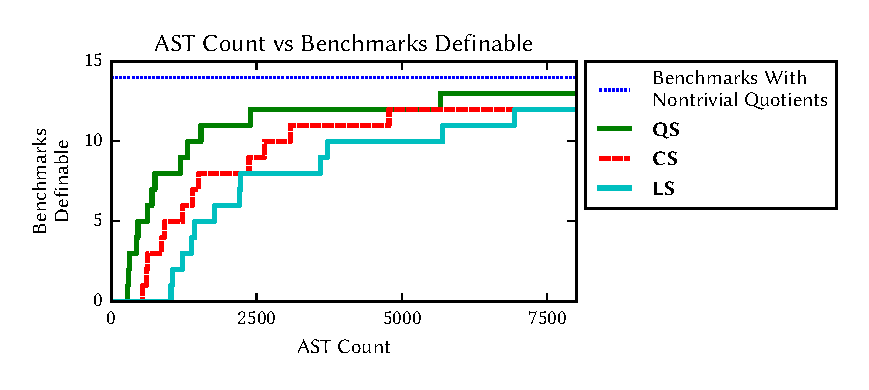
\includegraphics{generated-graphs/asts.eps}
\caption{Count of benchmark programs definable using a given AST count. We find
that it takes far fewer AST nodes to define benchmark lenses using QRE
synthesis than with Optician without QRE synthesis or without synthesis.\saz{Why
is the bar for ``All QRE Benchmarks'' at 14? Shouldn't it be at 47 = 39+8? Are
we not testing all QRE benchmarks?}}
\label{fig:asts}
\end{figure}

To get a sense of how much the new expressiveness that combining QRE lenses with
synthesis saves in terms of programmer effort, we compared the amount of code
that would need to be written for each of the lens benchmarks.  We use number of
nodes in the abstract syntax tree as a measure of code size, and calculated
three quantities for each lens synthesis benchmark task.  \saz{Say something
  about why there are only 14 benchmarks?}
%
\begin{itemize}
  \item[\QRESize{}] the number of AST nodes in the QRE
  specifications (including examples)\saz{CHECK THIS}
  \item[\CanonizerAndSpecSize{}]  the number of
  AST nodes in $W(q)$ summed with the number of AST nodes in $\canonizer(q)$
  \item[\LensAndSpecSize{}] the number of AST nodes
  in $W(q)$ summed with the number of AST nodes in the synthesized QRE lens.
\end{itemize}

The value of \QRESize{} is our measure of the programmer burden for
writing our benchmarks---it measures the number of AST nodes the programmer has
to write using the full expressiveness of QREs and synthesis.

The value of \CanonizerAndSpecSize{} estimates the burden for writing our
benchmarks within the Optician system, without QREs but still using
synthesis. This is only an approximation, as both $W(q)$ and $\canonizer(q)$ are
automatically generated from the QRE, and it is possible that a human-written
version might be smaller.

The value of \LensAndSpecSize{} estimates the burden in writing our benchmarks
in Boomerang, using neither QREs nor synthesis. This value is also an
approximation, as $W(q)$ and $\canonizer(q)$ and the bijective lens are all
automatically generated.

Figure~\ref{fig:asts} shows the number of benchmarks that can be expressed using
at most a given number of AST nodes. For a given benchmark, we found \QRESize{}
to be about half as large as \CanonizerAndSpecSize, and about a third as large
as \LensAndSpecSize{}. This demonstrates that introducing QREs saves programmers
significant effort compared to both Optician and basic Boomerang.

\subsection{Increasing Expressivity}

The pre-QRE version of Optician was only able to synthesize fully bijective data
transformations.  Synthesizing from QREs loosens that restriction, making it
possible to synthesize data which is bijective when put in canonical form. To
determine the increase of expressivity, we analyzed:
\begin{enumerate}
  \item How many data formats in Optician's benchmark suite required modifications
  to be bijective.
  \item How many data formats in Optician's benchmark suite required modifications
  to be bijective when put in canonical form.
\end{enumerate}

We found that 10 of Optician's 39 benchmarks required modifications to be
bijective. We found that 4 of Optician's 39 benchmarks required modifications to
be in bijective correspondence when in canonical form.\saz{Is this somehow where
  the 14 = 10+4 points in Fig. 10 come from?}\saz{Do these 10 and 4 intersect?}
Furthermore, we found that all eight of the data.gov examples required no
modifications to be in bijective correspondence when in canonical form. While we
did not put the data.gov examples into a form suitable for pre-QRE Optician, we
found that only four of the eight data.gov examples did not require
canonization, so making them suitable for pre-QRE Optician would have required 
changes to of four of the data.gov formats.  Here again, we see that QREs add
significant expressive power.

\subsection{Maintaining Competitive Performance}

\begin{figure}[t]
\centering
\begin{subfigure}[b]{.49\textwidth}
\centering
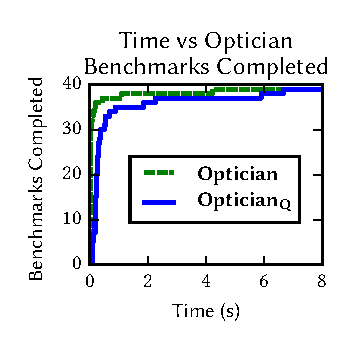
\includegraphics{generated-graphs/times_opt}
\caption{}
\label{subfig:lenssize}
\end{subfigure}
\begin{subfigure}[b]{.49\textwidth}
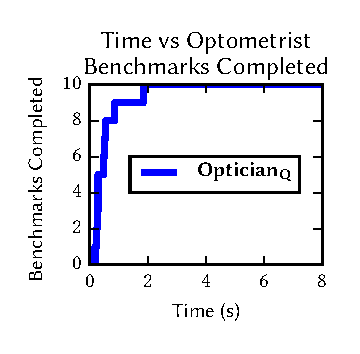
\includegraphics{generated-graphs/times_new.eps}
\caption{}
\label{subfig:examplesused}
\end{subfigure}
\caption{Runtimes of Optician and our system.
In (a), we run Optician and our system on Optician's benchmarks.  We find that
there is only a negligible difference incurred by Optometrist's overhead.
In (b), we run Optometrist on its benchmark suite.  We find that it is able
to synthesize all quotient lenses in under 20 seconds, and typically
finished in under 5 seconds. }
\label{fig:times}
\end{figure}

To assess the performance impact of adding QRE support to Optician, we measured
the running time of the following configurations:
\begin{itemize}
  \item[\OpticianRuntime{}] pre-QRE Optician running on its own benchmarks.
  \item[\SystemOnOptician{}] Optician with QREs running on the pre-QRE benchmarks.
  \item[\SystemOnBenchmarks{}] Optician with QREs running on its own benchmarks.
\end{itemize}

We summarize the results of these experiments in Figure~\ref{fig:times}.  The
new version of Optician was able to synthesize all of pre-QRE Optician's
benchmarks at a speed competitive with the old version.  There is a small amount
of additional overhead introduced by QREs when calculating $W(q)$ and $K(q)$,
resulting in a very slight decrease in performance.

Also notable is one of the data.gov examples, which converts demographic
statistics by zip code from xml form into rdf form. This took longer because it
was an exceptionally large format, converting over 40 fields.\saz{We need to
  explain more detail here.  I guess this is about the last benchmark in Fig. 11
  (b), which takes a long time?}  We added in additional fields to make this
format suitable for Optician, which took over 15 seconds synthesize the modified
lens.\saz{This needs more context, explanation.}

\section{Related Work}
\label{relwork}

\iffalse
Bidirectional transformations have been used in diverse areas of computing
where they arise as parsers and pretty printers, marshallers
and unmarshallers, serializers and deserializers, database views and view
updaters and many others\sam{TODO put citations}. Such transformations have
been extensively studied since they were proposed as a solution to the classical
{\em view-update problem} in the database community, where the challenge is to
derive a program that extracts a view of data from a source, as well as a
program that folds view updates back into the source safely and correctly.
\fi
This paper builds on the work of Foster et al~\cite{quotientlenses} who
introduced the theory of quotient lenses and implemented quotient lenses as a
refinement of the bidirectional string processing language Boomerang.
In Boomerang, the source and target types are specified using regular
expressions, and the equivalence relations are expressed using canonizers, which
are functions that map elements of a regular language to their canonical
representative. Boomerang canonizers can express a very broad class of
equivalence relations between regular languages, but actually doing so is often
difficult with complicated equivalence relations. For instance, Boomerang's
in-build permutation combinator does not account for separators in between the
regular expressions. Also, this combinator permutes regular expressions rather
than canonizers, thus making it difficult to express nested permutations that
occur in many data formats, especially XML and XML-like formats.

In their paper, Foster et al also discuss other bidirectional programming
languages that support quotienting of data including XSugar~\cite{xsugar},
biXid~\cite{bixid} and X/Inv~\cite{Hu2004,Mu2004,Mu2006}. XSugar programs
bidirectionally convert data stored in XML and ASCII formats respectively, with the
transformations specified by a pair of unambiguous grammars. The quotienting
occurs on the XML side by use of a generic canonizer that standardizes the
representation of trees. Well-formed XSugar programs are guaranteed to be
bijective modulo an equivalence relation that captures XML normalization. biXid
programs convert between pairs of XML documents, with the XML formats specified
using a pair of grammars as in XSugar. However, biXid grammars can be ambiguous.
This ambiguity is what allows biXid to express equivalences on the data.
Finally, Foster et al discuss a possible connection with the languages
X and Inv which support a primitive duplication combinator that does not work
well with the lens laws, but can be expressed using Boomerang quotient lenses.

As far as synthesis goes, though there is a good deal of recent research on
synthesizing unidirectional string
transformations~\cite{singh2012learning,le-pldi-2014,gulwani-popl-2014,perelman2014test,Singh:blinkfill},
the system Optician, which we introduced in ~\cite{optician}, is the first attempt
to synthesize bidirectional transformations that we are aware of. In that
publication, we compared Optician to two of these unidirectional string
transformers, Flash Fill~\cite{gulwani-popl-2014} and
FlashExtract~\cite{le-pldi-2014}, and found that these tools were unsuccessful
in synthesizing the complex transformatiunons that can be expressed in Optician.

While Optician improved on prior effors at synthesizing unidirectional string
transformers and introduced synthesis for bidirectional string transformations,
Optician was only able to synthesize fully bijective data transformations. Our
new system \Name{} improves on Optician in that \Name{} loosens this
restriction, and is able to synthesize data which is bijective when put in
canonical form. \Name{} is therefore a refinement of Optician since the
new synthesis algorithm (i.e. the quotient lens synthesis algorithm) restricted
to ``pure'' regular expressions degenerates to the synthesis algorithm that
we introduced in Optician. Indeed, as we mentioned in the evaluation section,
\Name{} was able to synthesize all of Optician's benchmarks at a speed
competitive with Optician, though there was additional overhead in calculating
the whole language $W(c)$ and the kernel language $K(c)$ of QREs, which
resulted in a very slight decrease in performance.

Much of the research in synthesis assumes that the synthesizer is provided with
a collection of examples. Optician and Optometrist differ in that they requires
that the programmer supplies both examples {\em and} format descriptions in the
form of regular expressions or QREs.  There is a trade-off here.  On the one
hand, a user must have some programming expertise to write regular expression
(or QRE) specifications and it requires some work. On the other hand, such
specifications provide a great deal of information to the synthesis system,
which decreases the number of examples needed (often to zero), makes the system
scale well, and allows it to handle large, complex formats.  By providing these
format specifications, the synthesis engine does not have to both infer the
format of the data as well as the transformations on it, obviating the need to
infer tricky formats like those involving nested iterations. Furthermore, by
focusing on bidirectional transformations, we limit the space of synthesized
functions to bijective ones, reducing the search space, and the expressiveness
of the search space.

There are many other recent results showing how to synthesize functions from
type-based
specifications~\cite{augustsson-2004,osera+:pldi15,feser-pldi-2015,scherer-icfp-2015,frankle+:popl16,armando+:pldi16}.
These systems enumerate programs of their target language, orienting their
search procedures to process only terms that are well-typed.
Optician is distinctive in that it synthesizes terms in a language with many
type equivalences.
Perhaps the system most similar to Optician is InSynth~\cite{gvero-pldi-2013}, a
system for synthesizing terms in the simply-typed lambda calculus that addresses
equivalences on types. Instead of trying to directly synthesize terms of the
simply-typed lambda calculus, InSynth synthesizes a well-typed term
in the succinct calculus, a language with types
that are equivalent ``modulo isomorphisms of products and
currying''~\cite{gvero-pldi-2013}. The type structure that we used in Optician
is significantly more complex.  In particular, because Optician types do not
have full canonical forms, we used a pseudo-canonical form, which captures part
of the equivalence relation over types. To preserve completeness, we pushed
some of the remaining parts of the type equivalence relation into a set of
rewriting rules and other parts into the synthesis algorithm itself.

Morpheus~\cite{morpheus} is another synthesis system that uses two
communicating synthesizers to generate programs.  In both Morpheus and
Optician, one synthesizer provides an
outline for the program, and the other fills in that outline with program
details that satisfy the user's specifications.
This approach works well in large search spaces that require some enumerative
search.
One important way that Optician differs from Morpheus is that in
Morpheus, an outline is a sketch---an
\emph{expression}
containing holes---whereas
an outline in Optician is a pair of regular
expressions, i.e., a
\emph{type}.  Moreover, in order to implement an efficient
search procedure, we had to create both a new type language and a new
term language for lenses.  Once we did so, we proved our new, more
constrained language
designed for synthesis was just as expressive as the original, more
flexible and compositional language designed for human programmers.

\section{Conclusion}
\bcp{And future work!}  \saz{I'm lukewarm about including a description of
future work.  Unless there are specific conjectures or open problems that
are worth mentioning, I'm not sure that it's really that important.}
\bcp{Agreed. But don't we have any ideas for how to extend or generalize or
things to do next??  E.g., is it completely trivial to extend all this to
asymmetric and symmetric lenses?  (If so, we should say so!)  Do we have
more ideas for QRE primitives?  Etc.}
\label{concl}

\bibliographystyle{plain}
\bibliography{local}


\end{document}
